\chapter{Testing Properties of Distributions: Lower Bounds from Reductions}\label{chap:unified:lb}

\epigraph{(``That's exactly the method,'' the Bellman bold\\
In a hasty parenthesis cried,\\
``That's exactly the way I have always been told\\
That the capture of Snarks should be tried!'')}{Lewis Carroll, \textit{The Hunting of the Snark}}

%%%%%%%%%%%%%%%%%%%%%%%%%%%%%%%%%%%%%%%%%%%%%%%%%%%%%%%%%%%%%%%%%%%%%%%%%%%%%%%%%%%%%%%%%%%%%%%%%%%%%%%%%%%%%%%%%%%%%%%%%%%%%%%%%%%%%%%%%%%%%%%%%%%%%%%

In spite of the considerable interest distribution testing has experienced in recent years, our arsenal of tools for proving lower bounds on the sample complexity of testing problems remains sorely limited. There are only a handful of standard techniques to prove such hardness results; and indeed the vast majority of the lower bounds in the literature are shown via \emph{Le Cam's two-point method} (also known as the ``easy direction'' of Yao's minimax principle)~\cite{Yu:97,Pollard:2003}.\footnote{In this method, one first defines two distributions $\dyes$ and $\dno$ over distributions that are respectively \yes-instances (having the property) and \no-instances (far from having the property). Then it remains to show that with high probability over the choice of the instance, every tester that can distinguish between $\p^{\yes} \sim \dyes$ and $\p^{\no} \sim \dno$ must use at least a certain number of samples.}{} In view of this scarcity, there has been in recent years a trend towards trying to obtain more, or simpler to use, techniques~\cite{Valiant:11,DK:16}; however, this state of affairs largely remains the same.

In this chapter, we set out to remedy this situation, by providing two general frameworks to establish distribution testing lower bounds. As we shall see, both are \emph{reduction-based} frameworks -- put differently, general techniques enabling us to capitalize on someone else's hard work from a different setting or area, and carry over their impossibility results to our distribution testing problem.
\begin{itemize}
  \item \cref{sec:learningreductions} describes our first reduction, which establishes a simple criterion under which hardness of testing a subproperty $\property'\subseteq \property$ carries over to testing $\property$ itself. This intuitive and seemingly ``obvious'' result -- \emph{``testing a class is at least as hard as testing anything it contains''} -- turns out to be false in general, as is easy to see even for some trivial cases. To remedy this unfortunate state of affairs, we identify a relatively benign assumption sufficient to make it hold; and show how this assumption is satisfied by a large number of natural properties.

  \item In~\cref{sec:communication}, we reveal a connection between distribution testing and the simultaneous message passing communication model, leading to our second methodology for proving distribution testing lower bounds. Extending the property testing lower bound framework of Blais, Brody, and Matulef~\cite{BBM:12}, we show a simple way of reducing communication problems to distribution testing ones. (Or, in other words, how to harness Alice and Bob's communication issues in order to prove distribution testing lower bounds.)
\end{itemize}
As an application, these two reduction-based approaches will allow us to show in a clean and painless fashion that most of the upper bounds obtained in~\cref{chap:unified:ub} are optimal or near-optimal, and cannot be significantly improved upon. In an unexpected turn of events, our second reduction will also reveal a connection between distribution testing and the field of interpolation theory, shedding light on an ``instance-optimal'' testing result of Valiant and Valiant~\cite{VV:14}.

%%%%%%%%%%%%%%%%%%%%%%%%%%%%%%%%%%%%%%%%%%%%%%%%%%%%%%%%%%%%%%%%%%%%%%%%%%%%%%%%%%%%%%%%%%%%%%%%%%%%%%%%%%%%%%%%%%%%%%%%%%%%%%%%%%%%%%%%%%%%%%%%%%%%%%%

\section{The Agnostic Learning Reduction}\label{sec:learningreductions}
We now turn to proving converses to our positive results -- namely, that many of the upper bounds we obtain cannot be significantly improved upon. As in our algorithmic approach, we describe for this purpose a \emph{generic framework} for obtaining lower bounds.

In order to state our results, we will require the usual definition of \emph{agnostic learning}. Recall that an algorithm is said to be a \emph{semi-agnostic learner} for a class \class if it satisfies the following. Given sample access to an arbitrary distribution $\D$ and parameter $\eps$, it outputs a hypothesis $\hat{\D}$ which (with high probability) does ``almost as well as it gets'':
\[
	\normone{\D - \hat{\D}} \leq c\cdot\opt_{\class,\D} + \bigO{\eps}
\]
where $\opt_{\class,\D}\eqdef \inf_{\D^\prime\in\class} \lp[1](\D^\prime,\D)$, and $c\geq 1$ is some absolute constant (if $c=1$, the learner is said to be agnostic).

\paragraph{High-level idea.} The motivation for our result is the observation of~\cite{BKR:04} that ``monotonicity is at least as hard as uniformity.'' Unfortunately, their specific argument does not generalize easily to other classes of distributions, making it impossible to extend it readily. The starting point of our approach is to observe that while uniformity testing is hard in general, it becomes very easy \emph{under the promise that the distribution is monotone, or even only close to monotone} (namely, $\bigO{1/\eps^2}$ samples suffice.)\footnote{Indeed, it is not hard to show that a monotone distribution can only be \eps-far from uniform if it puts probability weight $1/2+\bigOmega{\eps}$ on the first half of the domain. Estimating this probability weight to an additive $O(\eps)$ is thus sufficient to conclude.} This can give an alternate proof of the lower bound for monotonicity testing, via a different reduction: first, test if  the unknown distribution is monotone; if it is, test whether it is uniform, now assuming closeness to monotone.

More generally, this idea applies to any class \class which \textsf{(a)} contains the uniform distribution, and \textsf{(b)} for which we have a $\littleO{\sqrt{n}}$-sample agnostic learner $\Learner$, as follows.
Assuming we have a tester $\Tester$ for $\class$ with sample complexity $\littleO{\sqrt{n}}$, define a uniformity tester as below.
\begin{itemize}
  \item test if $\D\in\class$ using $\Tester$; if not, reject (as $\uniform\in\class$, $\D$ cannot be uniform);
  \item otherwise, agnostically learn $\D$ with $\Learner$ (since $\D$ is close to $\class$), and obtain hypothesis $\hat{\D}$;
  \item check offline if $\hat{D}$ is close to uniform.
\end{itemize} 
By assumption, $\Tester$ and $\Learner$ each use $\littleO{\sqrt{n}}$ samples, so does the whole process; but this contradicts the lower bound of~\cite{BFRSW:00,Paninski:08} on uniformity testing. Hence, $\Tester$ must use $\bigOmega{\sqrt{n}}$ samples.\medskip

This ``testing-by-narrowing'' reduction argument can be further extended to other properties than to uniformity, as we show below:
\begin{theorem}\label{theo:main:testing:lb}
Let \class be a class of distributions over $[n]$ for which the following holds:
\begin{enumerate}[(i)]
  \item there exists a semi-agnostic learner $\Learner$ for $\class$, with sample complexity $q_L(n,\eps, \delta)$ and ``agnostic constant''~$c$;
  \item there exists a subclass $\class_{\rm Hard}\subseteq\class$ such that testing $\class_{\rm Hard}$ requires $q_H(n,\eps)$ samples.
\end{enumerate}
Suppose further that $q_L(n,\eps, 1/6)=\littleO{q_H(n,\eps)}$. Then, any tester for $\class$ must use $\bigOmega{q_H(n,\eps)}$ samples.
\end{theorem}
\begin{proof}
The above theorem relies on the reduction outlined above, which we rigorously detail here. Assuming $\class$, $\class_{\rm Hard}$, $\Learner$ as above (with semi-agnostic constant $c \geq 1$), and a tester $\Tester$ for \class with sample complexity $q_T(n,\eps)$, we define a tester $\Tester_{\rm Hard}$ for $\class_{\rm Hard}$. On input $\eps\in(0,1]$ and given sample access to a distribution $\D$ on $[n]$, $\Tester_{\rm Hard}$ acts as follows:
\begin{itemize}
  \item call $\Tester$ with parameters $n$, $\frac{\eps^\prime}{c}$ (where $\eps^\prime\eqdef\frac{\eps}{3}$) and failure probability $1/6$, to $\frac{\eps^\prime}{c}$-test if $\D\in\class$. If not, reject.
  \item otherwise, agnostically learn a hypothesis $\hat{\D}$ for $\D$, with $\Learner$ called with parameters $n$, $\eps^\prime$ and failure probability $1/6$;
  \item check offline if $\hat{\D}$ is $\eps^\prime$-close to $\class_{\rm Hard}$, accept if and only if this is the case.
\end{itemize} 
We condition on both calls (to $\Tester$ and $\Learner$) to be successful, which overall happens with probability at least $2/3$ by a union bound. The completeness is immediate: if $\D\in\class_{\rm Hard}\subseteq\class$, $\Tester$ accepts, and the hypothesis $\hat{\D}$ satisfies $\normone{\hat{\D}-\D} \leq \eps^\prime$. Therefore, $\lp[1](\hat{\D},\class_{\rm Hard}) \leq \eps^\prime$, and $\Tester_{\rm Hard}$ accepts.

For the soundness, we proceed by contrapositive. Suppose $\Tester_{\rm Hard}$ accepts; it means that each step was successful. In particular, $\lp[1](\hat{\D},\class)\leq {\eps^\prime}/{c}$; so that the hypothesis outputted by the agnostic learner satisfies $\normone{\hat{\D}-\D} \leq c\cdot\opt+\eps^\prime\leq 2\eps^\prime$. In turn, since the last step passed and by a triangle inequality  we get, as claimed, $\lp[1](\D, \class_{\rm Hard}) \leq 2\eps^\prime + \lp[1](\hat{\D},\class_{\rm Hard}) \leq 3\eps^\prime = \eps$.

Observing that the overall sample complexity is $q_T(n,\frac{\eps^\prime}{c})+q_L(n,\eps^\prime, \frac{1}{6}) = q_T(n,\frac{\eps^\prime}{c})+\littleO{q_H(n,\eps^\prime)}$ concludes the proof.
\end{proof}

Taking $\class_{\rm Hard}$ to be the singleton consisting of the uniform distribution, and from the semi-agnostic learners of~\cite{CDSS:13,CDSS:14} (each with sample complexity either $\poly(1/\eps)$ or $\poly(\log n,1/\eps)$), we obtain the following:\footnote{Specifically, these lower bounds hold as long as $\eps=\bigOmega{1/n^\alpha}$ for some absolute constant $\alpha > 0$ (so that the sample complexity of the agnostic learner is indeed negligible in front of $\sqrt{n}/\eps^2$).}
\corolbsqrtn*
Similarly, we can use another result of~\cite{DDS:PBD:12} which shows how to agnostically learn Poisson Binomial Distributions with $\tildeO{1/\eps^2}$ samples.\footnote{Note the quasi-quadratic dependence on $\eps$ of the learner, which allows us to get $\eps$ into our lower bound for $n\gg \poly\log(1/\eps)$.} Taking $\class_{\rm Hard}$ to be the single $\binomial{n}{1/2}$ distribution (along with the testing lower bound of~\cite{VV:14}), this yields the following:
\corolbpbd*

\noindent Finally, we derive a lower bound on testing $k$-SIIRVs from the agnostic learner of~\cite{DDDOST:13} (which has sample complexity $\poly(k,1/\eps)$, independent~of~$n$):
\corolbksiirv*
\begin{proofof}{\cref{coro:lb:ksiirv}}
To prove this result, it is enough by \cref{theo:main:testing:lb} to exhibit a particular $k$-SIIRV $S$ such that testing identity to $S$ requires this many samples. Moreover, from~\cite{VV:14} this last part amounts to proving that the (truncated) 2/3-norm $\norm{S^{-\max}_{-\eps}}_{2/3}$ of $S$ is $\bigOmega{k^{1/2}n^{1/4}}$ (for every $\eps\in(0,\eps_0)$, for some small $\eps_0>0$). Our hard instance $S$ will be defined as follows: it is defined as the distribution of $X_1+\dots+X_n$, where the $X_i$'s are independent integer random variables uniform on $\{0,\dots,k-1\}$ (in particular, for $k=2$ we get a $\binomial{n}{1/2}$ distribution). It is straightforward to verify that $\shortexpect{S} = \frac{n(k-1)}{2}$ and $\sigma^2\eqdef\var S = \frac{(k^2-1)n}{12} = \bigTheta{k^2 n}$; moreover, $S$ is log-concave (as the convolution of $n$ uniform distributions). From this last point, we get that \textsf{(i)} the maximum probability of $S$, attained at its mode, is $\norminf{S}=\bigTheta{1/\sigma}$; and \textsf{(ii)} for every $j$ in an interval $I$ of length $2\sigma$ centered at this mode, $S(j) \geq \bigOmega{\norminf{S}}$ (see e.g.~\cite[Lemma 5.7]{DKS:15:arXiv} for the latter point). Define now $\eps_0$ as an absolute constant such that  $2\eps_0 \leq \D(I) = \bigOmega{1}$.

We want to lower bound $\norm{S^{-\max}_{-\eps}}_{2/3}$, for $\eps\leq \eps_0$; as by the above the ``$-\max$'' part can only change the value by $\norminf{S}=o(1)$, we can ignore it. Turning to the $-\eps$ part, i.e. the removal of the $\eps$ probability mass of the elements with smallest probability, note that this can only result in zeroing out at most $\frac{\eps}{\D(I)}\abs{I}\leq \frac{1}{2}\abs{I}$ elements in $I$ (call these $J_\eps\subseteq I$). From this, we obtain that
\[
    \norm{S^{-\max}_{-\eps}}_{2/3}\geq \Big(\sum_{j\in I\setminus J_\eps} S(j)^{2/3}\Big)^{3/2} \geq \mleft(\frac{1}{2}\cdot 2\sigma\cdot \bigOmega{1/\sigma}^{2/3}\mright)^{3/2} =\bigOmega{\sigma^{1/2}} = \bigOmega{k^{1/2}n^{1/4}}
\]
which concludes the proof.
\end{proofof}

\subsection{Tolerant Testing}\label{sec:lowerbounds:tol}

This lower bound framework from the previous section carries to \emph{tolerant} testing as well, resulting in this analogue to~\cref{theo:main:testing:lb}:
\begin{theorem}\label{theo:main:testing:tol:lb}
Let \class be a class of distributions over $[n]$ for which the following holds:
\begin{enumerate}[(i)]
  \item there exists a semi-agnostic learner $\Learner$ for $\class$, with sample complexity $q_L(n,\eps, \delta)$ and ``agnostic constant''~$c$;
  \item there exists a subclass $\class_{\rm Hard}\subseteq\class$ such that \emph{tolerant} testing $\class_{\rm Hard}$ requires $q_H(n,\eps_1,\eps_2)$ samples for some parameters $\eps_2 > (4c+1)\eps_1$.
\end{enumerate}
Suppose further that $q_L(n,\eps_2-\eps_1, 1/10)=\littleO{q_H(n,\eps_1,\eps_2)}$. Then, any \emph{tolerant} tester for $\class$ must use $\bigOmega{q_H(n,\eps_1,\eps_2)}$ samples (for some explicit parameters $\eps^\prime_1,\eps^\prime_2$).
\end{theorem}
\begin{proof}
The argument follows the same ideas as for \cref{theo:main:testing:lb}, up to the details of the parameters. Assuming $\class$, $\class_{\rm Hard}$, $\Learner$ as above (with semi-agnostic constant $c \geq 1$), and a tolerant tester $\Tester$ for \class with sample complexity $q(n,\eps_1,\eps_2)$, we define a tolerant tester $\Tester_{\rm Hard}$ for $\class_{\rm Hard}$. On input $0 < \eps_1 < \eps_2 \leq 1$ with $\eps_2 > (4c+1)\eps_1$, and given sample access to a distribution $\D$ on $[n]$, $\Tester_{\rm Hard}$ acts as follows. After setting $\eps^\prime_1\eqdef\frac{\eps_2-\eps_1}{4}$, $\eps^\prime_2\eqdef\frac{\eps_2-\eps_1}{2}$, $\eps^\prime \eqdef \frac{\eps_2-\eps_1}{16}$ and $\tau\eqdef \frac{6\eps_2+10\eps_1}{16}$,
\begin{itemize}
  \item call $\Tester$ with parameters $n$, $\frac{\eps^\prime_1}{c}$, $\frac{\eps^\prime_2}{c}$ and failure probability $1/6$, to tolerantly test if $\D\in\class$. If $\lp[1](\D,\class) > \eps^\prime_2/c$, reject.
  \item otherwise, agnostically learn a hypothesis $\hat{\D}$ for $\D$, with $\Learner$ called with parameters $n$, $\eps^\prime$ and failure probability $1/6$;
  \item check offline if $\hat{\D}$ is $\tau$-close to $\class_{\rm Hard}$, accept if and only if this is the case.
\end{itemize} 
We condition on both calls (to $\Tester$ and $\Learner$) to be successful, which overall happens with probability at least $2/3$ by a union bound. We first argue completeness: 
assume $\lp[1](\D,\class_{\rm Hard}) \leq \eps_1$. This implies $\lp[1](\D,\class) \leq \eps_1$, so that $\Tester$ accepts as $\eps_1 \leq \eps^\prime_1/c$ (which is the case because $\eps_2 > (4c+1)\eps_1$). Thus, the hypothesis $\hat{\D}$ satisfies $\normone{\hat{\D}-\D} \leq c\cdot \eps^\prime_1/c + \eps^\prime = \eps^\prime_1 + \eps^\prime$. Therefore, 
  $\lp[1](\hat{\D},\class_{\rm Hard}) \leq \normone{\hat{\D}-\D} + \lp[1](\D,\class_{\rm Hard}) \leq \eps^\prime_1 + \eps^\prime + \eps_1 < \tau$, and $\Tester_{\rm Hard}$ accepts.

For the soundness, we again proceed by contrapositive. Suppose $\Tester_{\rm Hard}$ accepts; it means that each step was successful. In particular, $\lp[1](\hat{\D},\class)\leq {\eps^\prime_2}/{c}$; so that the hypothesis outputted by the agnostic learner satisfies $\normone{\hat{\D}-\D} \leq c\cdot\opt+\eps^\prime\leq \eps^\prime_2 + \eps^\prime$. In turn, since the last step passed and by a triangle inequality  we get, as claimed, 
$\lp[1](\D, \class_{\rm Hard}) \leq \eps^\prime_2 + \eps^\prime + \lp[1](\hat{\D},\class_{\rm Hard}) \leq \eps^\prime_2 + \eps^\prime + \tau < \eps_2$.

Observing that the overall sample complexity is $q_T(n,\frac{\eps^\prime_1}{c},\frac{\eps^\prime_2}{c})+q_L(n,\eps^\prime, \frac{1}{10}) = q_T(n,\frac{\eps^\prime}{c})+\littleO{q_H(n,\eps^\prime)}$ concludes the proof.
\end{proof}

As before, we instantiate the general theorem to obtain specific lower bounds for tolerant testing of the classes we covered in this paper. That is, taking $\class_{\rm Hard}$ to be the singleton consisting of the uniform distribution (combined with the tolerant testing lower bound of~\cite{ValiantValiant:10lb} (restated in~\cref{theo:samp:uniformity:tolerant}), which states that tolerant testing of uniformity over $[n]$ requires $\bigOmega{\frac{n}{\log n}}$ samples), and again from the semi-agnostic learners of~\cite{CDSS:13,CDSS:14} (each with sample complexity either $\poly(1/\eps)$ or $\poly(\log n,1/\eps)$), we obtain the following:
\corolbtolnlogn*
Similarly, we again turn to the class of Poisson Binomial Distributions, for which we can invoke as before the $\tildeO{1/\eps^2}$-sample agnostic learner of~\cite{DDS:PBD:12}. As before, we would like to choose for $\class_{\rm Hard}$ the single $\binomial{n}{1/2}$ distribution; however, as no tolerant testing lower bound for this distribution exists~--~to the best of our knowledge~--~in the literature, we first need to establish the lower bound we will rely upon:

\begin{restatable}{theorem}{binomialtolerantlbtheorem}\label{theo:samp:binomial:tolerant:lb}
    There exists an absolute constant $\eps_0>0$ such that the following holds. Any algorithm which, given sampling access to an unknown distribution $\D$ on $\domain$ and parameter $\eps \in (0,\eps_0)$, distinguishes with probability at least $2/3$ between \textsf{(i)} $\normone{\D-\binomial{n}{1/2}} \leq \eps$ and \textsf{(ii)} $\normone{\D-\binomial{n}{1/2}} \geq 100\eps$ must use $\bigOmega{\frac{1}{\eps}\frac{\sqrt{n}}{\log n}}$ samples.
\end{restatable}
The proof relies on a reduction from tolerant testing of \emph{uniformity}, drawing on a result of Valiant and Valiant~\cite{ValiantValiant:10lb}; and is deferred to~\cref{app:binomial:tolerant:lb}. With~\cref{theo:samp:binomial:tolerant:lb} in hand, we can apply~\cref{theo:main:testing:tol:lb} to obtain the desired lower bound:
\corolbtolpbd*

\noindent We observe that both~\cref{coro:tol:lb:nlogn} and~\cref{coro:lb:tol:pbd} are tight (with regard to the dependence on $n$), as proven in the next section (\cref{sec:toltesting:ub}).\cmargin{Fix this reference.}

\subsubsection{Proof of~\cref{theo:samp:binomial:tolerant:lb}}\label{app:binomial:tolerant:lb}
The theorem will be a consequence of the (slightly) more general result below:
\begin{theorem}\label{theo:samp:binomial:tolerant}
  There exist absolute constants $\eps_0> 0$ and $\lambda > 0$ such that the following holds. Any algorithm which, given sample access to an unknown distribution $\D$ on $\domain$ and parameter $\eps \in (0,\eps_0)$, distinguishes with probability at least $2/3$ between \textsf{(i)} $\normone{\D-\binomial{n}{\frac{1}{2}}} \leq \eps$ and \textsf{(ii)} $\normone{\D-\binomial{n}{\frac{1}{2}}} \geq \lambda\eps^{1/3}-\eps$ must use $\bigOmega{\eps\frac{\sqrt{n}}{\log(\eps n)}}$ samples.
\end{theorem}
\noindent By choosing a suitable $\eps$ and working out the corresponding parameters, this for instance enables us to derive the following:
\begin{corollary}\label{coro:samp:binomial:tolerant}
  There exists an absolute constant $\eps_0 \in(0,1/1000)$ such that the following holds. Any algorithm which, given sample access to an unknown distribution $\D$ on $\domain$, distinguishes with probability at least $2/3$ between \textsf{(i)} $\normone{\D-\binomial{n}{\frac{1}{2}}} \leq \eps_0$ and \textsf{(ii)} $\normone{\D-\binomial{n}{\frac{1}{2}}} \geq 100\eps_0$ must use $\bigOmega{\frac{\sqrt{n}}{\log n}}$ samples.
\end{corollary}
\begin{proofof}{\cref{coro:samp:binomial:tolerant}}
The corollary follows from the proof of~\cref{theo:samp:binomial:tolerant}, by choosing $\eps_0>0$ sufficiently small so that $\frac{\lambda\eps_0^{1/3}-\eps_0}{\eps_0} \geq 100$.
\end{proofof}
\noindent By standard techniques, this will in turn imply~\cref{theo:samp:binomial:tolerant:lb}.\footnote{Namely, for $\eps\in(0,\eps_0)$, define the  mixture $\D_\eps \eqdef \frac{\eps}{\eps_0}\D+(1-\frac{\eps}{\eps_0})\binomial{n}{1/2}$. Being able to distinguish $\normone{\D_\eps-\binomial{n}{1/2}} \leq \eps$ from $\normone{\D_\eps-\binomial{n}{1/2}} \geq 100\eps$ in $q$ samples then allows one to distinguish $\normone{\D-\binomial{n}{1/2}} \leq \eps_0$ from $\normone{\D-\binomial{n}{1/2}} \geq 100\eps_0$ in $O(\eps\cdot q)$ samples.}

\begin{proofof}{\cref{theo:samp:binomial:tolerant}}
Hereafter, we write for convenience $B_n\eqdef \binomial{n}{\frac{1}{2}}$. To prove this lower bound, we will rely on the following:
\begin{theorem}[{\cite[Theorem 1]{ValiantValiant:10lb}}]\label{theo:samp:uniformity:tolerant}
  For any constant $\phi\in(0,1/4)$, following holds. Any algorithm which, given sample access to an unknown distribution $\D$ on $\{1,\dots,N\}$, distinguishes with probability at least $2/3$ between \textsf{(i)} $\normone{\D - \uniform_N} \leq \phi$ and \textsf{(ii)} $\normone{\D - \uniform_N} \geq \frac{1}{2}-\phi$, must have sample complexity at least $\frac{\phi}{32}\frac{N}{\log N}$.
\end{theorem}

Without loss of generality, assume $n$ is even (so that $B_n$ has only one mode located at $\frac{n}{2}$). For $c>0$, we write $I_{n,c}$ for the interval $\{\frac{n}{2}-c\sqrt{n},\dots,\frac{n}{2}+c\sqrt{n}\}$ and $J_{n,c}\eqdef\domain\setminus I_{n,c}$.
\begin{fact}\label{fact:easy:binomial}
For any $c > 0$, \[
\frac{B_n(\frac{n}{2} + c\sqrt{n})}{B_n({n}/{2})}, \frac{B_n(\frac{n}{2} - c\sqrt{n})}{B_n({n}/{2})} \operatorname*{\sim}_{n\to\infty} e^{-2c^2} \]
and 
\[
B_n(I_{n,c}) \in (1\pm o(1))\cdot[e^{-2c^2},1]\cdot 2c\sqrt{\frac{2}{\pi}} = \bigTheta{c}\,.
\]
\end{fact}

The reduction proceeds as follows: given sampling access to $\D$ on $[N]$, we can simulate sampling access to a distribution $\D^\prime$ on $[n]$ (where $n=\bigTheta{N^2}$) such that
\begin{itemize}
  \item if $\normone{\D - \uniform_N} \leq \phi$, then $\normone{\D^\prime - B_n} < \eps$;
  \item if $\normone{\D - \uniform_N} \geq \frac{1}{2}-\phi$, then $\normone{\D^\prime - B_n} > \eps^\prime - \eps$
\end{itemize}
for $\eps \eqdef \Theta(\phi^{3/2})$ and $\eps^\prime \eqdef \Theta(\phi^{\frac{1}{2}})$; in a way that preserves the sample complexity. The high-level idea is that (by the above fact) the Binomial distribution over $\domain$ is almost uniform on the middle $O(\sqrt{n})$ elements, and has a constant fraction of its probability mass there: we can therefore ``embed'' the tolerant uniformity testing lower bound (for support $O(\sqrt{n})$) into this middle interval.\smallskip

More precisely, define $c\eqdef \sqrt{\frac{1}{2}\ln\frac{1}{1-\phi}} =\bigTheta{\sqrt{\phi}}$ (so that $\phi = 1 - e^{-2c^2}$) and $n$ such that $\abs{I_{n,c}}= N$ (that is, $n=(N/(2c))^2 = \bigTheta{N^2/\phi}$). From now on, we can therefore identify $[N]$ to $I_{n,c}$ in the obvious way, and see a draw from $\D$ as an element in $I_{n,c}$.

Let $p\eqdef B_n(I_{n,c}) = \bigTheta{\sqrt{\phi}}$, and $B_{n,c}$, $\bar{B}_{n,c}$ respectively denote the conditional distributions induced by $B_n$ on $I_{n,c}$ and $J_{n,c}$. Intuitively, we want $\D$ to be mapped to the conditional distribution of $\D^\prime$ on $I_{n,c}$, and the conditional distribution of $\D^\prime$ on $J_{n,c}$ to be exactly $\bar{B}_{n,c}$. This is achieved by defining $\D^\prime$ by the process below:
\begin{itemize}
  \item with probability $p$, we draw a sample from $\D$ (seen as an element of $I_{n,c}$);
  \item with probability $1-p$, we draw a sample from $\bar{B}_{n,c}$.
\end{itemize}
Let $\tilde{B}_n$ be defined as the distribution which exactly matches $B_n$ on $J_{n,c}$, but is uniform on $I_{n,c}$:
\begin{align*}
  \tilde{B}_n(i) = \begin{cases}
    \frac{p}{\abs{I_{n,c}}} & i\in I_{n,c}\\
    B_n(i) & i\in J_{n,c}\\
     \end{cases}
\end{align*}
From the above, we have that $\normone{\D^\prime - \tilde{B}_n} = p\cdot \normone{\D - \uniform_N}$. Furthermore, by \cref{fact:easy:binomial}, \cref{lemma:small:l2:close:uniform:l1} and the definition of $I_{n,c}$, we get that $\normone{B_n - \tilde{B}_n} = p\cdot \normone{(B_n)_{I_{n,c}} - \uniform_{I_{n,c}}} \leq p\cdot \phi$. Putting it all together,

\begin{itemize}
  \item If $\normone{\D - \uniform_N} \leq \phi$, then by the triangle inequality $\normone{\D^\prime - B_n} \leq p(\phi + \phi) = 2p\phi$;
  \item If $\normone{\D - \uniform_N} \geq \frac{1}{2}-\phi$, then similarly $\normone{\D^\prime - B_n} \geq p(\frac{1}{2}-\phi -\phi) = \frac{p}{4}-2p\phi$.
\end{itemize}
Recalling that $p= \bigTheta{\sqrt{\phi}}$ and setting $\eps \eqdef 2p\phi$ concludes the reduction. From~\cref{theo:samp:uniformity:tolerant}, we conclude that
\[
\frac{\phi}{32}\frac{N}{\log N}
  = \bigOmega{\phi\frac{\sqrt{\phi n}}{\log(\phi n)}} 
  = \bigOmega{\eps\frac{\sqrt{n}}{\log(\eps n)}}
\]
samples are necessary.
\end{proofof}


\section{The Communication Complexity Reduction}\label{sec:communication}
%%%%%%%%%%%%%%%%%%%%%%%%%%%%%%%%%%%%%%%%%%%%%%%%%%%%%%%%%%%%%%%%%%%%%%%%%%%%%%%%%%%%%%%%%%%%%%%%%%%%%%%%%%%%%%%%%%%%%%%%%%%%%%%%%%%%%%%%%%%%%%%%%%%%%%%
\subsection{Introduction}\label{sec:introduction:communication}
% Distribution testing, as first explicitly introduced in~\cite{BFRSW:00}, is a branch of property testing~\cite{RS:96,GGR:98} concerned with the study of sublinear algorithms for making approximate decisions regarding probability distributions over massive domains. These algorithms are granted access to independent samples from an unknown distribution and are required to \emph{test} whether this distribution has a certain global property. That is, a tester for property $\Pi$ of distributions over domain $\Omega$ receives a proximity parameter $\eps>0$ and is asked to determine whether a distribution $\p$ over $\Omega$ (denoted $\p\in\distribs{\Omega}$) has the property $\Pi$ or is $\eps$-far (say, in $\lp[1]$-distance) from any distribution that has $\Pi$, using a small number of independent samples from $\p$. The \emph{sample complexity} of $\Pi$ is then the minimal number of samples needed to test it. Throughout the introduction, we fix $\eps$ to be small constant and refer to a tester with respect to proximity parameter $\eps$ as an \emph{$\eps$-tester}.

As the reader may have picked up from the previous chapters,\todonote{Is that OK to say?}{} distribution testing has been studied extensively in recent years. In a significant body of work spanning more than a decade~\cite{BFFKRW:01,Paninski:04,BDKR:05,Paninski:08,ADJOP:11,BFRV:11,LRR:13,VV:14,CDVV:14,WY:14,JVW:14,BV:15,DK:16}, a myriad of properties has been investigated under this lens. Starting with~\cite{GRexp:00,BFRSW:10,BFFKRW:01}, this includes the testing of symmetric properties~\cite{RRSS:09,Valiant:11,VV:11:stoc,ValiantValiant:11}, of structured families~\cite{BKR:04,ILR:12,AD:15,Canonne:15,ADK:15,CDGR:16,Canonne:16}, as well as testing under some assumption on the unknown instance~\cite{RS:09,DDSVV:13,DKN:15,DKN:15:FOCS}. Tight upper and lower bounds on the sample complexity have been obtained for properties such as uniformity, identity to a specified distribution, monotonicity, and many more (see references above, or~\cite{Rubinfeld:12:Survey,Canonne:15:Survey} for surveys).
 However, while by now numerous techniques and approaches are available to design distribution testers, our arsenal of tools for proving lower bounds on the sample complexity of distribution testing is significantly more limited. There are only a handful of standard techniques to prove lower bounds; and indeed the vast majority of the lower bounds in the literature are shown via \emph{Le Cam's two-point method} (also known as the ``easy direction'' of Yao's minimax principle)~\cite{Yu:97,Pollard:2003}. In this method, one first defines two distributions $\dyes$ and $\dno$ over distributions that are respectively \yes-instances (having the property) and \no-instances (far from having the property). Then it remains to show that with high probability over the choice of the instance, every tester that can distinguish between $\p^{\yes} \sim \dyes$ and $\p^{\no} \sim \dno$ must use at least a certain number of samples. In view of this scarcity, there has been in recent years a trend towards trying to obtain more, or simpler to use, techniques~\cite{Valiant:11,DK:16}; however, this state of affairs largely remains the same.

In this work, we reveal a connection between distribution testing and the simultaneous message passing ($\SMP$) communication model, which in turn leads to a new methodology for proving distribution testing lower bounds. Recall that in a private-coin $\SMP$ protocol, Alice and Bob are given strings $x,y \in \bitset^k$ (respectively), and each of the players is allowed to send a message to a referee (which depends on the player's input and private randomness) who is then required to decide whether $f(x,y)=1$ by only looking at the players' messages and flipping coins.

\begin{figure}[ht]\centering
  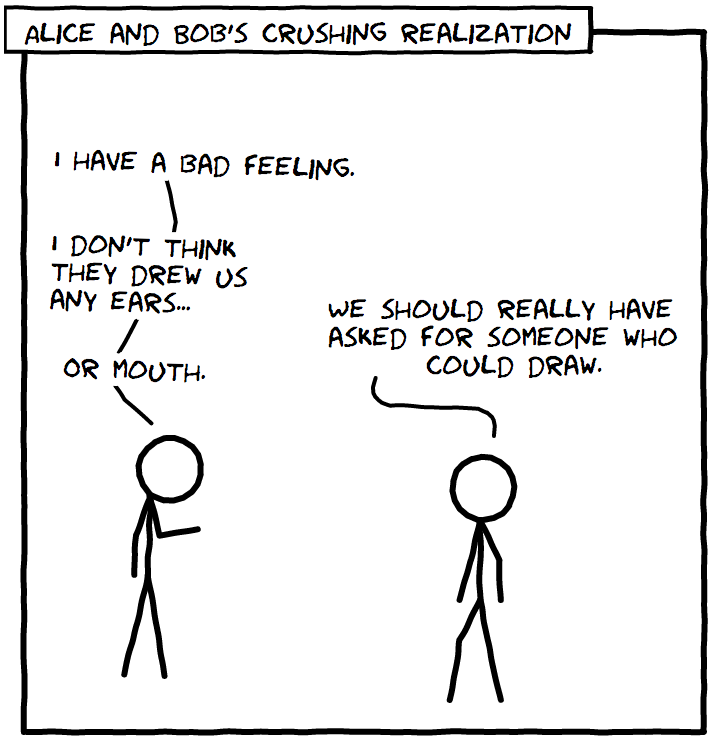
\includegraphics[width=0.5\textwidth]{chapter2/fig-alicebob}
  \caption{Communicating has been somewhat hard for Alice and Bob lately.}
\end{figure}

Extending the framework of Blais, Brody, and Matulef~\cite{BBM:12}, we show a simple way of reducing (private-coin) $\SMP$ problems to distribution testing problems. This foregoing methodology allows us to prove new distribution testing lower bounds, as well as to provide simpler proofs of known lower bounds for problems such as testing uniformity, monotonicity, and $k$-modality (see~\cref{sec:other}). 

Our main result is a characterization of the sample complexity of the distribution identity testing problem in terms of a key operator in the study of interpolation spaces, which arises naturally from our reduction and for which we are able to provide an intuitive interpretation. Recall that in this problem, the goal is to determine whether a distribution $\q$ over domain $\Omega$ (denoted $\q\in\distribs{\Omega}$) is identical to a fixed distribution $\p$; that is, given a full description of $\p\in\distribs{\Omega}$, we ask how many independent samples from $\q$ are needed to decide whether $\q=\p$, or whether $\q$ is $\eps$-far in $\lp[1]$-distance from $\p$.\footnote{Note that this is in fact a family of massively parameterized properties $\{\Pi_p\}_{p\in\distribs{\Omega}}$, where $\Pi_p$ is the property of being identical to $\p$. See~\cite{Newman:10} for an excellent survey concerning massively parameterized properties.}

% \newcommand{\pb}[2]{\parbox[c][][c]{#1}{\strut#2\strut}}
  \begin{table}[ht]\centering\small
    \begin{adjustwidth}{-.5in}{-.5in}\centering
    \def\arraystretch{1.5}   \begin{tabular}{@{}|l|c|c|@{}}\hline
    { \bf Property }& \textbf{Our results} & \bf Previous bounds\\\hline
    {Uniformity}  & $\tildeOmega{\sqrt{n}}$ 
                 & {$\bigTheta{\sqrt{n}}$ \cite{GRexp:00,Paninski:08}} \\\hline
     {Identity to $\p$}  & {$\bigOmega{\kf{\p}^{-1}(1-\eps)}, \bigO{\kf{\p}^{-1}(1-c\cdot\eps)}$ }
                 & {$\bigOmega{\norm{\p^{-\max}_{\eps}}_{2/3}}, \bigO{\norm{\p^{-\max}_{c'\cdot\eps}}_{2/3}}$ \cite{VV:14}} \\\hline
     {Monotonicity}  & $\tildeOmega{\sqrt{n}}$ 
                 & {$\bigTheta{\sqrt{n}}$ \cite{BKR:04,ADK:15,CDGR:16}} \\\hline
     {$k$-modal}  & $\tildeOmega{\sqrt{n}}$
                 & {$\tildeOmega{\max(\sqrt{n},k)}$ \cite{Canonne:16}} \\\hline
     \pb{42mm}{Log-concavity, Monotone Hazard Rate}  & $\tildeOmega{\sqrt{n}}$ 
                 & {$\bigTheta{\sqrt{n}}$ \cite{ADK:15,CDGR:16}} \\\hline
     \pb{42mm}{Binomial, Poisson Binomial}  & $\tildeOmega{{n}^{1/4}}$ 
                 & {$\bigTheta{{n}^{1/4}}$~(\cite{AD:15,CDGR:16}} \\\hline
     \pb{42mm}{Symmetric sparse support}  & $\tildeOmega{\sqrt{n}}$ 
                 & \cellcolor{gray!25}\\\hline
      \pb{42mm}{Junta distributions ($\PCOND$ model)}  & $\bigOmega{k}$ 
                 & \cellcolor{gray!25}\\\hline
  \end{tabular}
  \end{adjustwidth}
    \caption{\label{fig:table:secommunication:results} Summary of results. All the bounds are stated for constant proximity parameter $\eps$.}
  \end{table}
 
In a recent and influential work, Valiant and Valiant~\cite{VV:14} showed that the sample complexity of the foregoing question is closely related to the $\lp[2/3]$-quasinorm of $\p$, defined as $\norm{\p}_{2/3} = \big(\sum_{\omega \in \Omega} \abs{\p(\omega)}^{2/3}\big)^{3/2}$. That is, viewing a distribution $\p \in\distribs{\Omega}$ as an $\abs{\Omega}$-dimensional vector of probabilities, let $\p_{-\eps}^{-\max}$ be the vector obtained from $\p$ by zeroing out the largest entry as well as the set of smallest entries summing to $\eps$ (note that $\p_{-\eps}^{-\max}$ is no longer a probability distribution). Valiant and Valiant gave an $\eps$-tester\footnote{Throughout the introduction, we fix $\eps$ to be small constant and refer to a tester with respect to proximity parameter $\eps$ as an \emph{$\eps$-tester}.}{} for testing identity to $\p$ with sample complexity $O\big({\norm{\p_{-c \eps}^{-\max}}_{2/3}}\big)$, where $c>0$ is a universal constant, and complemented this result with a lower bound of $\Omega\big({\norm{\p_{-\eps}^{-\max}}_{2/3}}\big)$.\footnote{We remark that for certain $\p$'s, the asymptotic behavior of $\bigO{\norm{\p_{-c\eps}^{-\max}}_{2/3}}$ strongly depends on the constant $c$, and so it cannot be omitted from the expression. We further remark that this result was referred to by Valiant and Valiant  as ``instance-optimal identity testing'' as the resulting bounds are phrased as a function of the distribution $\p$ itself -- instead of the standard parameter which is the domain size $n$.}

In this work, using our new methodology, we show alternative and similarly tight bounds on the complexity of identity testing, in terms of a more intuitive measure (as we discuss below) and using simpler arguments. Specifically, we prove that the sample complexity is essentially determined by a fundamental quantity in the theory of interpolation of Banach spaces, known as Peetre's \emph{$K$-functional}. Formally, for a distribution $\p\in\distribs{\Omega}$, the $K$-functional between $\lp[1]$ and $\lp[2]$ spaces is the operator defined for $t>0$ by
\begin{equation*}
    \kf{\p}(t) = \inf_{\p'+ \p''=\p} \normone{\p'} + t\normtwo{\p''}.
\end{equation*}

This operator can be thought of as an interpolation norm between the $\lp[1]$ and $\lp[2]$ norms of the distribution $\p$ (controlled by the parameter $t$), naturally inducing a partition of $\p$ into two sub-distributions: $\p'$, which consists of ``heavy hitters'' in $\lp[1]$-norm, and $\p''$, which has a bounded $\lp[2]$-norm. Indeed, the approach of isolating elements with large mass and testing in $\lp[2]$-norm seems inherent to the problem of identity testing, and is the core component of both early works~\cite{GRexp:00,BFFKRW:01} and more recent ones~\cite{DKN:15,DK:16,Gol:16}. As a further connection to the identity testing question, we provide an easily interpretable proxy for this measure $\kf{\p}$, showing that the $K$-functional between the $\lp[1]$ and $\lp[2]$ norms of the distribution $\p$ is closely related to the size of the effective support of $\p$, which is the number of supported elements that constitute the vast majority of the mass of $\p$; that is, we say that $\p$ has \emph{$\eps$-effective support} of size $T$ if $1- O(\eps)$ of the mass of $\p$ is concentrated on $T$ elements (see~\cref{sec:overview:ub} for details).

Having defined the $K$-functional, we can proceed to state the lower bound we derive for the problem.\footnote{As stated, this result is a slight strengthening of our communication complexity reduction, which yields a lower bound of $\bigOmega{\kf{\p}^{-1}(1-2\eps)/\log n}$. This strengthening is described in~\cref{sec:id:lb}.}
\begin{theorem}[Informally stated]
\label{introthm:1}
Any $\eps$-tester of identity to $\p\in\distribs{\Omega}$ must have sample complexity $\bigOmega{\kf{\p}^{-1}(1-2\eps)}$.
\end{theorem}
\noindent 
In particular, straightforward calculations show that for the uniform distribution we obtain a tight lower bound of $\bigOmega{\sqrt{n}}$, and for the Binomial distribution we obtain a tight lower bound of $\bigOmega{n^{1/4}}$.

To show that tightness of the lower bound above, we complement it with a nearly matching upper bound, also expressed in terms of the $K$-functional.
\begin{theorem}[Informally stated]
\label{introthm:2}
There exist an absolute constant $c>0$ and an $\eps$-tester of identity to $\p\in\distribs{\Omega}$ that uses $\bigO{\kf{\p}^{-1}(1-c\eps)}$ samples.\footnote{Similarly to the~\cite{VV:14} bound, for certain $\p$'s, the asymptotic behavior of $\bigO{\kf{\p}^{-1}(1-2\eps)}$ depends on the constant $c$, and so it cannot be omitted from the expression.}
\end{theorem}
\noindent We remark that for some distributions the bounds in Theorems~\ref{introthm:1}~and~\ref{introthm:2} are tighter than the bounds in \cite{VV:14}, whereas for other distributions it is the other way around (see discussion in Section~\ref{sec:kfunctional}).

In the following section, we provide an overview of our new methodology as well as the proofs for the above theorems. We also further discuss the interpretability of the $K$-functional and show its close connection to the effective support size. We conclude this section by outlining a couple of extensions of our methodology.

\subparagraph{Dealing with sub-constant values of the proximity parameter.} Similarly to the communication complexity methodology for proving property testing lower bounds~\cite{BBM:12}, our method inherently excels in the regime of \emph{constant} values of the proximity parameter $\eps$. Therefore, in this work we indeed focus on the constant proximity regime. However, in~\cref{sec:eps_dep} we demonstrate how to obtain lower bounds that asymptotically increase as $\eps$ tends to zero, via an extension of our general reduction.


\subparagraph{Extending the methodology to testing with conditional samples.} Testers with sample access are by far the most commonly studied algorithms for distribution testing. However, many scenarios that arise both in theory and practice are not  fully captured by this model. In a recent line of works~\cite{CFGM:13,CRS:15,ACK:14,FJOPS:15,FLV:16}, testers with access to \emph{conditional} samples were considered, addressing situations in which one can control the samples that are obtained by requesting samples conditioned on membership on subsets of the domain. In~\cref{sec:extensions}, we give an example showing that it is possible to extend our methodology to obtain lower bounds in the conditional sampling model.

\subsubsection{Organization}
We first give a technical overview in~\cref{sec:technical_overview}, demonstrating the new methodology and presenting our bounds on identity testing. %\cref{sec:prelim} then provides the required preliminaries for the main technical sections. 
In~\cref{sec:methodology} we formally state and analyze the $\SMP$ reduction methodology for proving distribution testing lower bounds. In~\cref{sec:uniformity:communication}, we instantiate the basic reduction, obtaining a lower bound on uniformity testing, and in~\cref{sec:eps_dep} show how to extend the methodology to deal with sub-constant values of the proximity parameter. (We stress that~\cref{sec:eps_dep} is \emph{not} a prerequisite for the rest of the sections, and can be skipped at the reader's convenience.) In~\cref{sec:kfunctional} we provide an exposition to the $K$-functional and generalize inequalities that we shall need for the following sections. \cref{sec:instanceoptimal:identity} then contains the proofs of both lower and upper bounds on the problem of identity testing, in terms of the $K$-functional. In~\cref{sec:other}, we demonstrate how to easily obtain lower bounds for other distribution testing problems. Finally, in~\cref{sec:extensions} we discuss extensions to our methodology; specifically, we explain how to obtain lower bounds in various metrics, and show a reduction from communication complexity to distribution testing in the conditional sampling model.

%%%%%%%%%%%%%%%%%%%%%%%%%%%%%%%%%%%%%%%%%%%%%%%%%%%%%%%%%%%%%%%%%%%%%%%%%%%%%%%%%%%%%%%%%%%%%%%%%%%%%%%%%%%%%%%%%%%%%%%%%%%%%%%%%%%%%%%%%%%%%%%%%%%%%%%
\subsection{Technical Overview}
\label{sec:technical_overview}
In this section we provide an overview of the proof of our main result, which consists of new lower and upper bounds on the sample complexity of testing identity to a given distribution, expressed in terms of an intuitive, easily interpretable measure. To do so, we first introduce the key component of this proof, the methodology for proving lower bounds on distribution testing problems via reductions from SMP communication complexity. We then explain how the relation to the theory of interpolation spaces and the so-called $K$-functional naturally arises when applying this methodology to the identity testing problem.

 For the sake of simplicity, throughout the overview we fix the domain $\Omega = [n]$ and fix the proximity parameter $\eps$ to be a small constant. We begin in~\cref{sec:uniformity_overview} by describing a simple ``vanilla'' reduction for showing an $\tildeOmega{\sqrt{n}}$ lower bound on the complexity of testing that a distribution is uniform. Then, in~\cref{sec:overview:lb} we extend the foregoing approach to obtain a new lower bound on the problem of testing identity to a fixed distribution. This lower bound depends on the best rate obtainable by a special type of error-correcting codes, which we call \emph{$\p$-weighted codes}. In~\cref{sec:overview:detour}, we show how to relate the construction of such codes to concentration of measure inequalities for weighted sums of Rademacher random variables; furthermore, we discuss how the use of the \emph{$K$-functional}, an interpolation norm between $\lp[1]$ and $\lp[2]$ spaces, leads to stronger concentration inequalities than the ones derived by Chernoff bounds or the central limit theorem. Finally, in~\cref{sec:overview:ub} we establish nearly matching upper bounds for testing distribution identity in terms of this $K$-functional, using a proxy known as the $Q$-norm. We then infer that the sample complexity of testing identity to a distribution $\p$ is roughly determined by the size of the \emph{effective support} of $\p$ (which is, loosely speaking, the number of supported elements which together account for the vast majority of the mass of $\p$).

\subsubsection{Warmup: Uniformity Testing.} 
\label{sec:uniformity_overview}
Consider the problem of testing whether a distribution $\q\in\distribs{[n]}$ is the \emph{uniform distribution}; that is, how many (independent) samples from $\q$ are needed to decide whether $\q$ is the uniform distribution over $[n]$, or whether $\q$ is $\eps$-far in $\lp[1]$-distance from it. We reduce the SMP communication complexity problem of \emph{equality} to the distribution testing problem of uniformity testing.

 Recall that in a private-coin SMP protocol for equality, Alice and Bob are given strings $x,y \in \bitset^k$ (respectively), and each of the players is allowed to send a message to a referee (which depends on the player's input and private randomness) who is then required to decide whether $x=y$ by only looking at the players' messages and flipping coins.
 
 \begin{figure}[ht!]
  \centering
  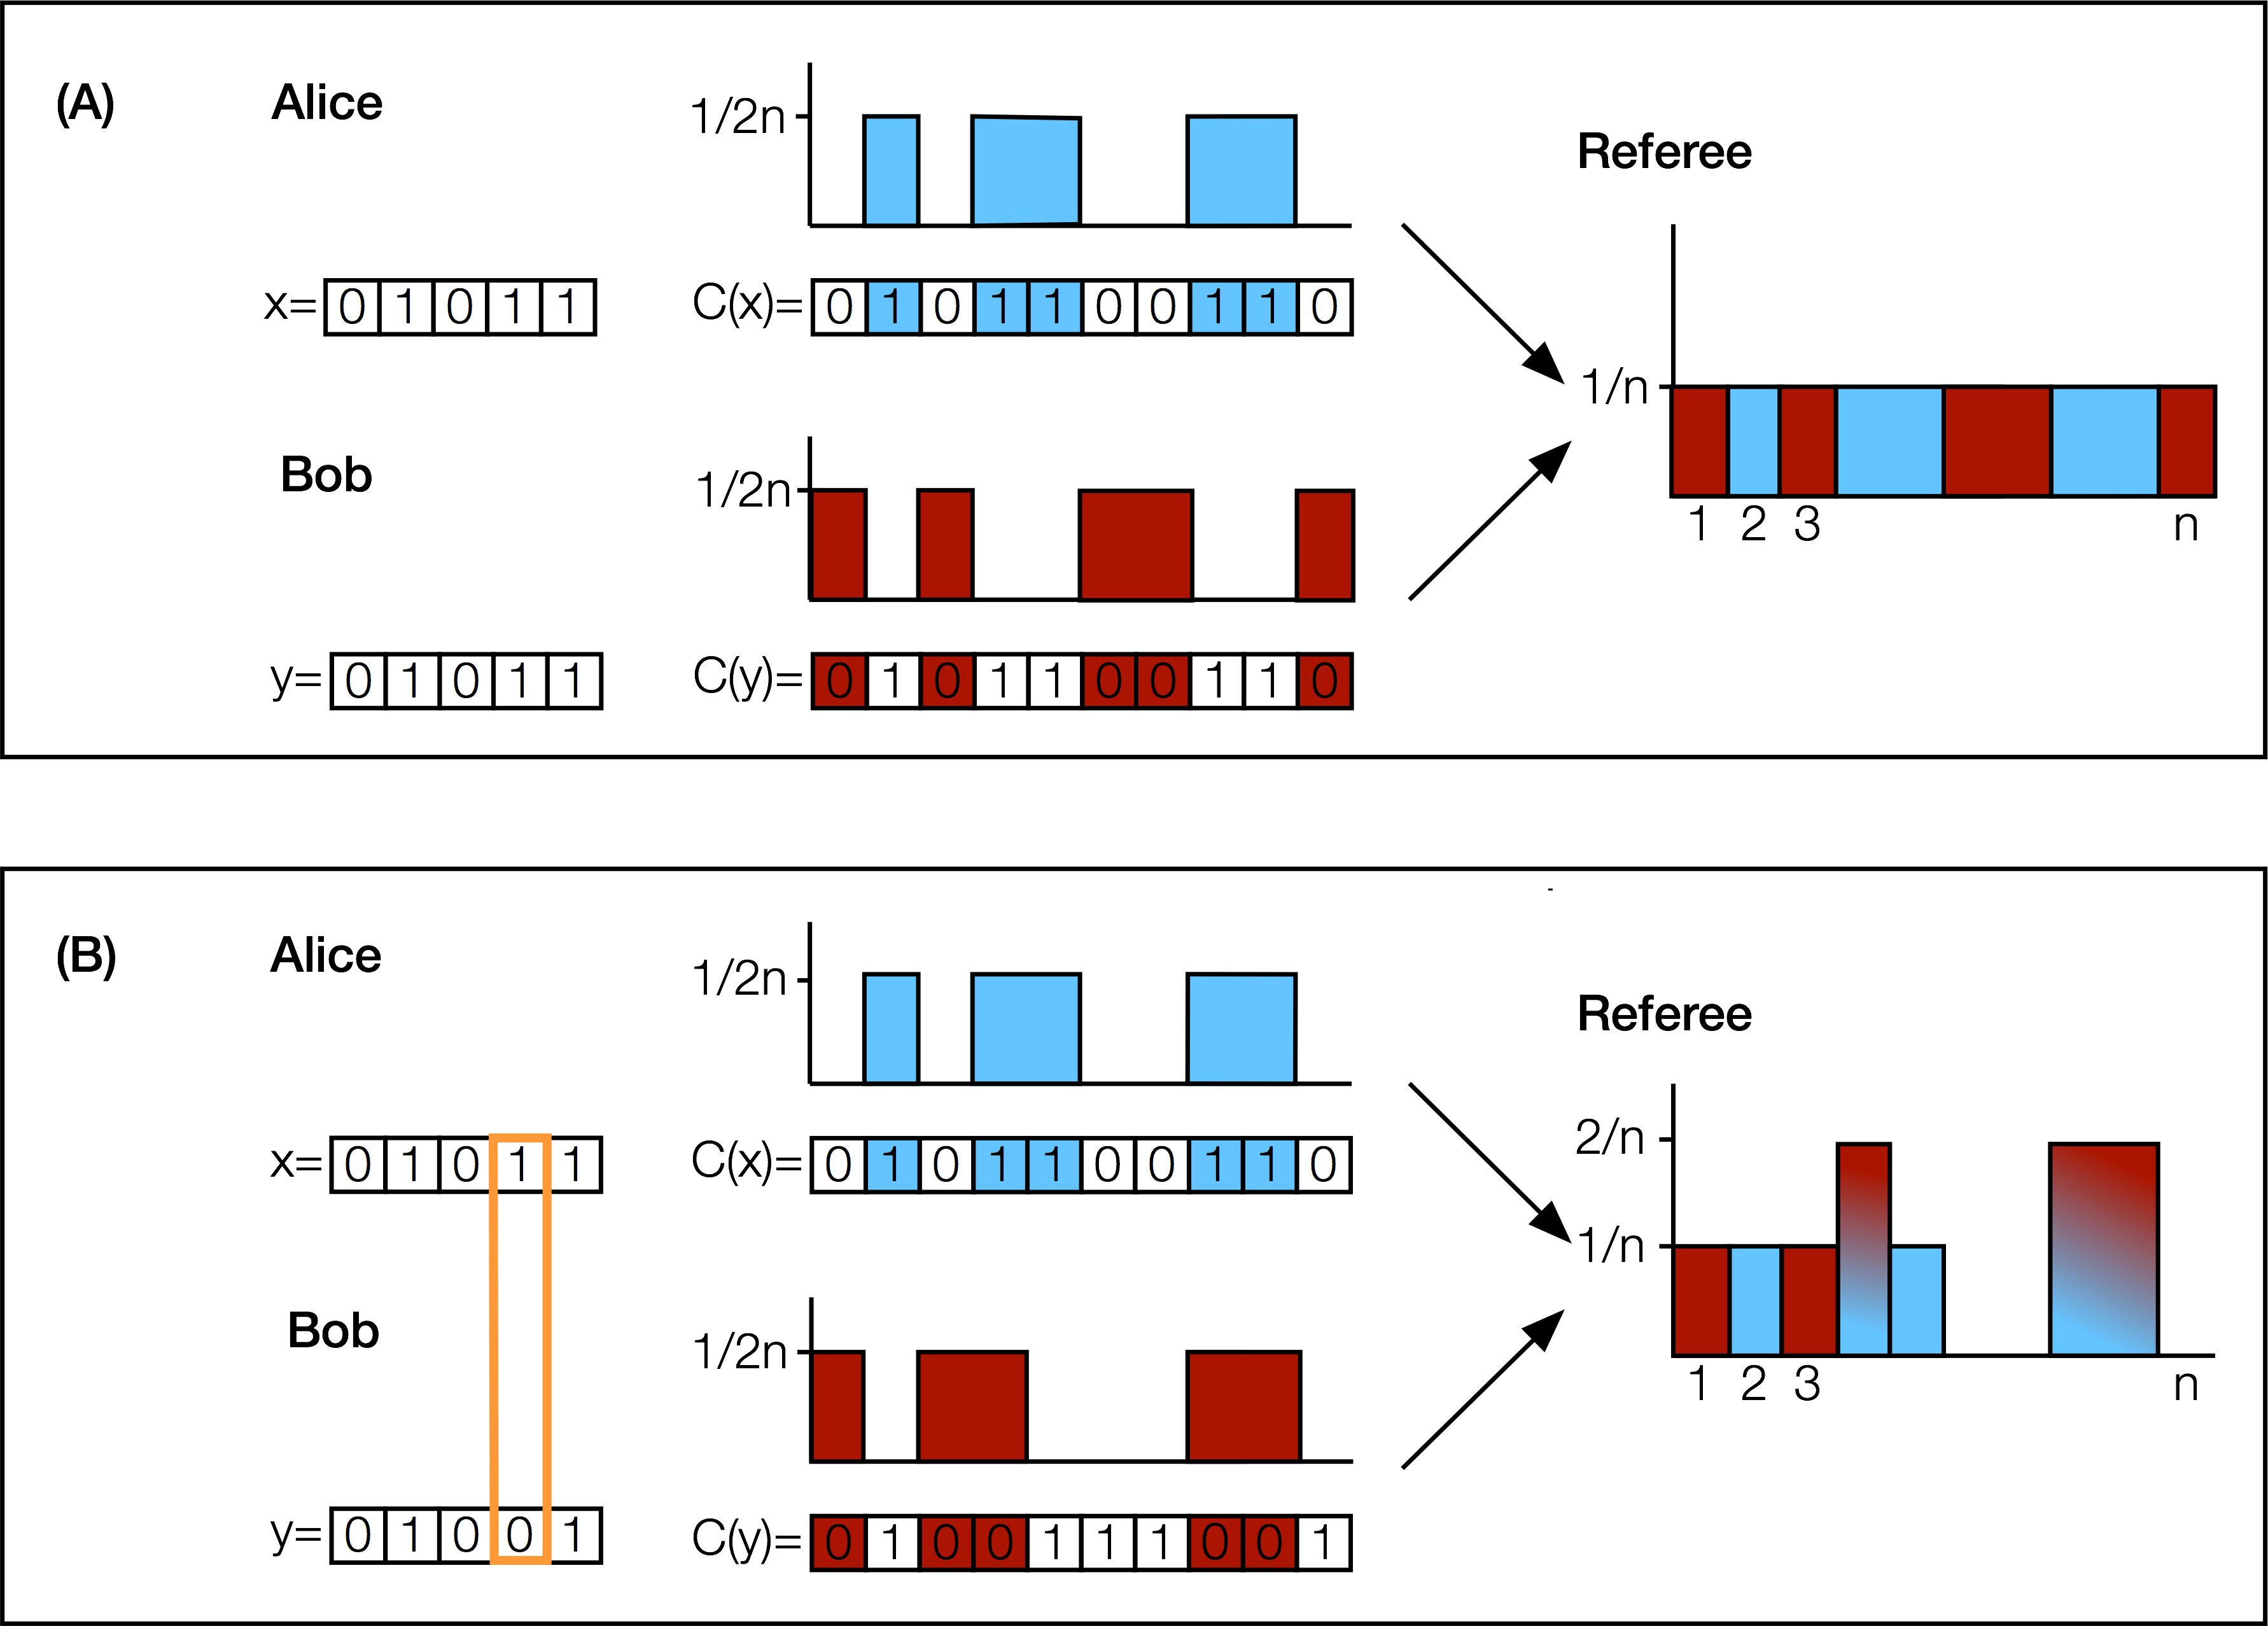
\includegraphics[scale=0.8]{chapter2/img_uniformity.png}
  \caption{{The reduction from equality in the SMP model to uniformity testing of distributions.} In (A) we see that the uniform distribution is obtained when $x=y$, whereas in (B) we see that when $x \neq y$, we obtain a distribution that is ``far'' from uniform.}
  \label{fig:uniformity}
\end{figure}

The reduction is as follows. Assume there exists a uniformity tester with sample complexity $s$. Each of the players encodes its input string via a balanced asymptotically good code $C$ (that is, $C\colon\bitset^k \to \bitset^n$ is an error-correcting code with constant rate and relative distance $\delta = \Omega(1)$, which satisfies the property that each codeword of $C$ contains the same number of $0$'s and $1$'s). Denote by $A \subset [n]$ the locations in which $C(x)$ takes the value $1$ (i.e., $A = \setOfSuchThat{ i\in[n] }{ C(x)_i = 1 }$), and denote by $B \subset [n]$ the locations in which $C(y)$ takes the value $0$ (i.e., $B = \setOfSuchThat{ i\in[n] }{ C(y)_i = 0 }$). Alice and Bob each send $\bigO{s}$ uniformly distributed samples from $A$ and $B$, respectively. Finally, the referee invokes the uniformity tester with respect to the distribution $\q= \left( \uniform_{A}+ \uniform_{B} \right)/2$, emulating each draw from $\q$ by tossing a random coin and deciding accordingly whether to use a sample by Alice or Bob. See~\cref{fig:uniformity}.

The idea is that if $x=y$, then $C(x)=C(y)$, and so $A$ and $B$ are a \emph{partition} of the set $[n]$. Furthermore, since $\abs{C(x)} = \abs{C(y)} = n/2$, this is a equipartition. Now, since Alice and Bob send uniform samples from an equipartition of $[n]$, the distribution $\q$ that the referee emulates is in fact the uniform distribution over $[n]$, and so the uniformity tester will accept. On the other hand, if $x\neq y$, then $C(x)$ and $C(y)$ disagree on a constant fraction of the domain. Thus, $A$ and $B$ intersect on $\delta/2$ elements, as well as do not cover $\delta/2$. Therefore $\q$ is uniform on a $(1-\delta)$-fraction of the domain, unsupported on a $(\delta/2)$-fraction of the domain, and has ``double'' weight $2/n$ on the remaining $(\delta/2)$-fraction. In particular, since $\delta = \bigOmega{1}$, the emulated distribution $\q$ is $\bigOmega{1}$-far (in $\lp[1]$-distance) from uniform, and it will be rejected by the uniformity tester.

As each sample sent by either Alice or Bob was encoded with $\bigO{\log n}$ bits, the above constitutes an SMP protocol for equality with communication complexity $O(s \log(n))$.  Yet it is well known~\cite{newman1996public} that the players must communicate $\Omega(\sqrt{k})$ bits to solve this problem (see~\cref{sec:methodology}), and so we deduce that $s = \Omega(\sqrt{k}/\log(n)) = \tilde\Omega(\sqrt{n})$.

\subsubsection{Revisiting Distribution Identity Testing: A New Lower Bound}
\label{sec:overview:lb}
Next, consider the problem of testing whether a distribution $\q\in\distribs{[n]}$ is identical to a fixed distribution $\p$, provided as a (massive) parameter; that is, given a full description of $\p\in\distribs{[n]}$, we ask how many independent samples from $\q$ are needed to decide whether $\q=\p$, or whether $\q$ is $\eps$-far in $\lp[1]$-distance from $\p$. As mentioned earlier, Valiant and Valiant~\cite{VV:14} established both upper and lower bounds on this problem, involving the $\lp[2/3]$-quasinorm of $\p$. We revisit this question, and show different -- and more interpretable -- upper and lower bounds. First, by applying our new communication complexity methodology to the distribution identity problem, we obtain a simple lower bound expressed in terms of a new parameter, which is closely related to the \emph{effective support size} of $\p$.

Consider any fixed $\p\in\distribs{[n]}$. As a first idea, it is tempting to reduce equality in the SMP model to testing identity to $\p$ by following the uniformity reduction described in~\cref{sec:uniformity_overview}, only instead of having Alice and Bob send \emph{uniform} samples from $A$ and $B$, respectively, we have them send samples from $\p$ \emph{conditioned} on membership in $A$ and $B$ respectively. That is, as before Alice and Bob encode their inputs $x$ and $y$ via a balanced, asymptotically good code $C$ to obtain the sets $A = \setOfSuchThat{ i\in[n] }{ C(x)_i = 1 }$ and $B = \setOfSuchThat{ i\in[n] }{ C(y)_i = 0 }$, which partition $[n]$ if $x=y$, and intersect on $\bigOmega{n}$ elements (as well as fail to cover $\bigOmega{n}$ elements of $[n]$) if $x \neq y$. Only now, Alice sends samples independently drawn from $\p|_A$, i.e., $\p$ conditioned on the samples belonging to $A$, and Bob sends samples independently drawn from $\p|_B$, i.e., $\p$ conditioned on the samples belonging to $B$; and the referee emulates the distribution $\q = (\p|_A + \p|_B)/2$.

However, two problems arise in the foregoing approach. The first is that while indeed when $x=y$ the reduction induces an equipartition $A,B$ of the domain, the resulting weights $\p(A)$ and $\p(B)$ in the mixture may still be dramatically different, in which case the referee will need much more samples from one of the parties to emulate $\p$. The second is a bit more subtle, and has to do with the fact that the properties of this partitioning are with respect to the \emph{size} of the symmetric difference $A\Delta B$, while really we are concerned about its \emph{mass} under the emulated distribution $\q$ (and although both are proportional to each other in the case of the uniform distribution, for general $\p$ we have no such guarantee). Namely, when $x \neq y$ the domain elements which are responsible for the  distance from $\p$ (that is, the elements which are covered by both parties ($A\cap B$) and by neither of the parties ($[n] \setminus (A\cup B)$) may only have a small mass according to $\p$, and thus the emulated distribution $\q$ will not be sufficiently far from $\p$. A natural attempt to address these two problems would be to preprocess $\p$ by discarding its light elements, focusing only on the part of the domain where $\p$ puts enough mass pointwise; yet this approach can also be shown to fail, as in this case the reduction may still not generate enough distance.\footnote{In more detail, this approach would consider the distribution $\p'$ obtained by iteratively removing the lightest elements of $\p$ until a total of $\eps$ probability mass was removed. This way, every element $i$ in the support of $\p'$ is guaranteed to have mass $\p'_i \geq \eps/n$: this implies that the weights $\p'(A)$ and $\p'(B)$ are proportional, and that each element that is either covered by both parties or not covered at all will contribute $\eps/n$ to the distance from $\p'$. However, the total distance of $\q$ from $\p$ would only be $\bigOmega{|\supp{\p'}| \cdot \eps/n}$; and this only suffices if $\p$ and $\p'$ have comparable support size, i.e. $|\supp{\p}| = \bigO{|\supp{\p'}|}$.}

Instead, we take a different route. The key idea is to consider a new type of codes, which we call \emph{$\p$-weighted codes}, which will allow us to circumvent the second obstacle. These are code whose distance guarantee is weighted according to the distribution $\p$; that is, instead of requiring that every two codewords $c,c'$ in a code $C$ satisfy $\dist{x}{y} \eqdef \sum_{i=1}^{n} \abs{ x_i - y_i } \geq \delta$, we consider a code $C_p\colon \bitset^k \to \bitset^n$ such that every $c,c' \in C_p$ satisfy
\[
    \pdist[\p]{x}{y} \eqdef \sum_{i=1}^{n} \p(i)\cdot\abs{ x_i - y_i } \geq \delta.
\]
Furthermore, to handle the first issue, we adapt the ``balance'' property accordingly, requiring that each codeword be balanced according to $\p$, that is, every $c \in C_p$ satisfies $\sum_{i=1}^{n} \p(i)\cdot c_i = 1/2$.

It is straightforward to see that if we invoke the above reduction while letting the parties encode their inputs via a balance $\p$-weighted code $C_p$, then both of the aforementioned problems are resolved; that is, by the $\p$-balance property the weights $\p(A)$ and $\p(B)$ are equal, and by the $\p$-distance of $C_p$ we obtain that for $x \neq y$ the distribution $\q = (\p_A + \p_B)/2$ is $\Omega(1)$-far from $\p$. Hence we obtain a lower bound of $\bigOmega{ \sqrt{k}/\log(n) }$ on the query complexity of testing identity to $\p$. To complete the argument, it remains to construct such codes, and determine what the best rate $k/n$ that can be obtained by $\p$-weighted codes is.

\subsubsection{Detour: $\p$-weighted Codes, Peetre's $K$-functional, and beating the CLT}
\label{sec:overview:detour}
The discussion of previous section left us with the task of constructing high-rate $\p$-weighted codes. Note that unlike standard (uniformly weighted) codes, for which we can easily obtain constant rate, there exist some $\p$'s for which high rate is impossible (for example, if $\p\in\distribs{[n]}$ is only supported on one element, we can only obtain rate $1/n$). In particular, by the sphere packing bound, every $\p$-weighted code $C\colon\bitset^k \to\bitset^n$ with distance $\delta$  must satisfy
\[
      \underbrace{2^k}_{\#\text{codewords}} \leq \frac{2^n}{\operatorname{Vol}_{\mathbb{F}_2^n,\pdistfunc[\p]}(\delta/2) },
\]
where $\operatorname{Vol}_{\mathbb{F}_2^n,\pdistfunc[\p]}(r)$ is the volume of the $\p$-ball of radius $r$ in the $n$-dimensional hypercube, given by
\[
 \operatorname{Vol}_{\mathbb{F}_2^n,\pdistfunc[\p]}(r) 
    \eqdef \abs{ \setOfSuchThat{w\in \mathbb{F}_2^n }{\sum_{i=1}^{n} \p_i\cdot w_i \leq r } }.
\]
Hence, we must have $k \leq n - \log \operatorname{Vol}_{\mathbb{F}_2^n,\pdistfunc[\p]}(\delta/2)$.

 In~\cref{sec:id:lb:cc} we show that there exist (roughly) balanced $\p$-weighted codes with nearly-optimal rate,\footnote{We remark that since these codes are not perfectly $\p$-balanced, a minor modification to the reduction needs to be done. See~\cref{sec:id:lb:cc} for details.} and so it remains to determine the volume of the $\p$-ball of radius $\eps$ in the $n$-dimensional hypercube, where recall that $\eps$ is the proximity parameter of the test. To this end, it will be convenient to represent this quantity as a concentration inequality of sums of weighted Rademacher random variables, as follows
   \begin{equation}
   \label{eq:Vol:overview}
    \operatorname{Vol}_{\mathbb{F}_2^n,\pdistfunc[\p]}(\eps)
        = 2^n \probaDistrOf{Y \sim \bitset^n }{ \sum_{i=1}^n \p_i Y_i \leq \eps } 
        = 2^n \probaDistrOf{X \sim \{-1,1\}^n }{ \sum_{i=1}^n \p_i X_i \geq 1-2\eps}. 
  \end{equation}
    Applying standard tail bounds derived from the central limit theorem (CLT), we have that
   \begin{equation}
   \label{eq:CLT}
 \probaDistrOf{X \sim \{-1,1\}^n }{ \sum_{i=1}^n \p_i X_i \geq 1-2\eps} \le e^{\frac{-(1-2\eps)^2}{2\normtwo{\p}^2}},
  \end{equation}
  and so we can obtain a $\p$-weighted code $C_p\colon\bitset^k \to \bitset^n$ with dimension $k = O(1/\normtwo{\p}^2)$, which in turn, by the reduction described in~\cref{sec:overview:lb}, implies a lower bound of $\bigOmega{1/(\normtwo{\p} \cdot \log(n))}$ on the complexity of testing identity to $\p$.
  
  Unfortunately, the above lower bound is not as strong as hoped, and in particular, far weaker than the $\norm{\p^{-\max}_{-\eps}}_{2/3}$ bound of~\cite{VV:14}.\footnote{For example, fix $\alpha \in (0,1)$, and consider the distribution $\p\in\distribs{[n]}$ in which $n/2$ elements are of mass $1/n$, and $n^{\alpha}/2$ elements are of mass $1/n^{\alpha}$. It is straightforward to verify that $\normtwo{\p}^{-1} = \bigTheta{(\sqrt{n})^{\alpha}}$, whereas $\norm{\p}_{2/3} = \bigTheta{\sqrt{n}}$. (Intuitively, this is because the $\lp[2]$-norm is mostly determined by the few heavy elements, whereas the $\lp[2/3]$-quasinorm is mostly determined by the numerous light elements.)} Indeed, it turns out that the CLT-based bound in~\cref{eq:CLT} is only tight for distributions satisfying $\norminf{\p} = O(\normtwo{\p}^2)$, and is in general too crude for our purposes.
   Instead, we look for stronger concentration of measure inequalities that ``beat'' the CLT. To this end, we shall use powerful tools from the theory of interpolation spaces. Specifically, we consider Peetre's \emph{$K$-functional} between $\lp[1]$ and $\lp[2]$ spaces. Loosely speaking, this is the operator defined for $t>0$ by
\begin{equation*}
    \kf{\p}(t) = \inf_{\p'+ \p'' =\p} \normone{\p'} + t\normtwo{\p''}.\footnotemark
\end{equation*}
\footnotetext{Interestingly, Holmstedt~\cite{Holm:70} showed that the infimum is \emph{approximately} obtained by partitioning $\p = (\p',\p'')$ such that $\p'$ consists of the heaviest $t^2$ coordinates of $\p$ and $\p''$ consists of the rest (for more detail, see~\cref{theo:bounds:kf}).}

This $K$-functional can be thought of as an interpolation norm between the $\lp[1]$ and $\lp[2]$ norms of the distribution $\p$ (and accordingly, for any fixed $t$ it defines a norm on the space $\lp[1]+\lp[2]$). In particular, note that for large values of $t$ the function $\kf{\p}(t)$ is close to $\normone{\p}$, whereas for small values of $t$ it will behave like $t\normtwo{\p}$.

The foregoing connection is due to Montgomery-Smith~\cite{MS:90}, who established the following concentration of measure inequality for weighted sums of Rademacher random variables,
\begin{equation}
\label{eq:Mont:overview}
  \probaOf{ \sum_{i=1}^n \p_i X_i \geq \kf{\p}(t) } \leq e^{-\frac{t^2}{2} }.
\end{equation}

Furthermore, he proved that this concentration bound is essentially tight (see~\cref{sec:kfunctional} for a precise statement). Plugging~\eqref{eq:Mont:overview} into~\eqref{eq:Vol:overview}, we obtain a lower bound of $\Omega(\kf{\p}^{-1}(1-2\eps)/\log(n))$ on the complexity of testing identity to $\p$.

To understand and complement this result, we describe in the next subsection a nearly tight upper bound for this problem, also expressed in terms of this $K$-functional; implying that this unexpected connection is in fact not a coincidence, but instead capturing an intrinsic aspect of the identity testing question. We also give a natural interpretation of this bound, showing that the size of the \emph{effective support} of $\p$ (roughly, the number of supported elements that constitute the vast majority of the mass of $\p$) is a good proxy for this parameter $\kf{\p}^{-1}(1-2\eps)$ -- and thus for the complexity of testing identity to $\p$.

\subsubsection{Using the $Q$-norm Proxy to Obtain an Upper Bound}
\label{sec:overview:ub}
To the end of obtaining an upper bound on the sample complexity of testing identity to $\p$, in terms of the $K$-functional, it will actually be convenient to look at a related quantity, known as the \emph{$Q$-norm}~\cite{MS:90}. At a high-level, the $Q$-norm of a distribution $\p$, for a given parameter $T\in\N$, is the maximum one can reach by partitioning the domain of $\p$ into $T$ sets and taking the sum of the $\lp[2]$ norms of these $T$ subvectors. That is
 \[
    \norm{\p}_{Q(T)} \eqdef \sup \setOfSuchThat{ \sum_{j=1}^T \left( \sum_{i\in A_j} \p_i^2 \right)^{1/2} }{ (A_j)_{1\leq j\leq T} \text{ partition of } \N }.
  \]

Astashkin~\cite{Astashkin:2010}, following up Montgomery-Smith~\cite{MS:90}, showed that the $Q$-norm constitutes a good approximation of $K$-functional, by proving that
  \begin{equation*}
    \norm{\p}_{Q(t^2)} \leq \kf{\p}(t) \leq \sqrt{2}\norm{\p}_{Q(t^2)}.
  \end{equation*}
In~\cref{sec:kfunctional} we further generalize this claim and show it is possible to get a tradeoff in the upper bound; specifically, we prove that
$\kf{\p}(t) \leq \norm{\p}_{Q(2t^2)}$. Thus, it suffices to prove an upper bound on distribution identity testing in terms of the $Q$-norm.

From an algorithmic point of view, it is not immediately clear that switching to this $Q$-norm is of any help. However, we will argue that this value captures -- in a very quantitative sense -- the notion of the \emph{sparsity} of $\p$. As a first step, observe that if $\norm{\p}_{Q(T)} = 1$, then the distribution $\p$ is supported on at most $T$ elements. To see this, denote by $\p_{A_j}$ the restriction of the sequence $\p$ to the indices in $A_j$, and note that if $\norm{\p}_{Q(T)} \eqdef \sum_{j=1}^T \normtwo{ \p_{A_j} }=1$, then  by the monotonicity of $\lp[p]$ norms and since $\sum_{j=1}^T \normone{ \p_{A_j} } = \normone{\p}=1$ we have that
\[
      \sum_{j=1}^T (\underbrace{ \normone{ \p_{A_j} } - \normtwo{ \p_{A_j} } }_{\geq 0}) = 0,
\]
which implies that $\normone{ \p_{A_j} } = \normtwo{ \p_{A_j} }$ for all $j\in[T]$.

Now, it turns out that it is possible to obtain a \emph{robust} version of the foregoing observation, yielding a sparsity lemma that, roughly speaking, shows thats if $\norm{\p}_{Q(T)} \geq 1-\eps$, then $1- O(\eps)$ of the mass of $\p$ is concentrated on $T$ elements: in this case we say that $\p$ has \emph{$O(\eps)$-effective support} of size $T$. (See \cref{lemma:ub:key} for precise statement of the sparsity lemma.)

 This property of the $Q$-norm suggests the following natural test for identity to a distribution $\p$: Simply fix $T$ such that  $\norm{\p}_{Q(T)} = 1-\eps$, and apply one of the standard procedures for testing identity to a distribution with support size $T$, which require $O(\sqrt{T})$ samples. But by the previous discussion, we have $\norm{\p}_{Q(2t^2)} \geq \kf{\p}(t)$, so that setting $T=2t^2$ for the ``right'' choice of $t=\kf{\p}^{-1}(1-2\eps)$ will translate to an $O(t)$ upper bound -- which is what we were aiming for.
 
%%%%%%%%%%%%%%%%%%%%%%%%%%%%%%%%%%%%%%%%%%%%%%%%%%%%%%%%%%%%%%%%%%%%%%%%%%%%%%%%%%%%%%%%%%%%%%%%%%%%%%%%%%%%%%%%%%%%%%%%%%%%%%%%%%%%%%%%%%%%%%%%%%%%%%%
\subsection{The Methodology: From Communication Complexity to Distribution Testing}\label{sec:methodology}
In this section we adapt the methodology for proving property testing lower bounds via reductions from communication complexity, due to Blais, Brody, and Matulef~\cite{BBM:12}, to the setting of distribution testing.  As observed in~\cite{BBM:12,BMW:11}, to prove lower bounds on the query complexity of \emph{non-adaptive} testers it suffices to reduce from one-sided communication complexity. We show that for distribution testers (which are inherently non-adaptive), it suffices to reduce from the more restricted communication complexity model of \emph{private-coin} simultaneous message passing (SMP).

Recall that a private-coin SMP protocol for a communication complexity predicate $f\colon \bitset^k \times \bitset^k \to \bitset$ consists of three computationally unbounded  parties: Two players (commonly referred to as Alice and Bob), and a Referee. Alice and Bob receive inputs $x,y \in \bitset^k$. Each of the players simultaneously (and independently) sends a message to the referee, based on its input and (private) randomness. The referee is then required to successfully compute $f(x,y)$ with probability at least $2/3$, using its private randomness and the messages received from Alice and Bob. The communication complexity of an SMP protocol is the total number of bits sent by Alice and Bob. The private-coin SMP complexity of $f$, denoted $\SMP(f)$, is the minimum communication complexity of all SMP protocols that solve $f$ with probability at least $2/3$.

Generally, to reduce an SMP problem $f$ to $\eps$-testing a distribution property $\Pi$, Alice and Bob can send  messages $m_A(x,r_A,\eps)$ and $m_B(y,r_B,\eps)$ (respectively) to the Referee, where $r_A$ and $r_B$ are the private random strings of Alice and Bob. Subsequently, the Referee uses the messages $m_A(x,r_A,\eps)$ and $m_A(y,r_B,\eps)$, as well as its own private randomness, to feed the property tester samples from a distribution $\p$ that satisfies the following conditions: (1) \emph{completeness}: if $f(x,y)=1$, then $\p\in \Pi$; and (2) \emph{soundness}: if $f(x,y)=0$, then $\p$ is $\eps$-far from $\Pi$ in $\ell_1$-distance.

We shall focus on a special type of the foregoing reductions, which is particularly convenient to work with and suffices for all of the our lower bounds. Loosely speaking, in these reductions Alice and Bob both send the prover samples from sub-distributions that can be combined by the Referee to obtain samples from a distribution that satisfies the completeness and soundness conditions. The following lemma gives a framework for proving lower bounds based on such reductions.

\begin{lemma}\label{lemma:main:methodology:reduction}
	Let $\eps>0$, and let $\Omega$ be a finite domain of cardinality $n$. Fix a property $\Pi \subseteq \distribs{\Omega}$ and a communication complexity predicate $f\colon \bitset^k \times \bitset^k \to \bitset$. Suppose that there exists a mapping $\p\colon\bitset^k \times \bitset^k \to \distribs{\Omega}$ that satisfies the following conditions.
	\begin{enumerate}
		\item \emph{Decomposability:} For every $x,y\in\bitset^k$, there exist constants $\alpha=\alpha(x), \beta=\beta(y) \in [0,1]$ and distributions $\p_A(x), \p_B(y)$ such that 
		\[
		p(x,y) = \frac{\alpha}{\alpha+\beta}\cdot \p_A(x) + \frac{\beta}{\alpha+\beta}\cdot \p_B(y)
		\] 
		and $\alpha,\beta$ can each be encoded with $\bigO{\log n}$ bits.
		\item \emph{Completeness:} For every $(x,y) = f^{-1}(1)$, it holds that $\p(x,y) \in \Pi$.
		\item \emph{Soundness:} For every $(x,y) = f^{-1}(0)$, it holds that $\p(x,y)$ is $\eps$-far from $\Pi$ in $\ell_1$ distance.
	\end{enumerate}
	Then, every $\eps$-tester for $\Pi$ needs $\bigOmega{\frac{\SMP(f)}{\log(n)}}$ samples.
\end{lemma}

\begin{proof}
Supose there exists an $\eps$-tester for $\Pi$ with sample complexity $s'$; assume without loss of generality that the soundness of the foregoing tester is $5/6$, at the cost of increasing the query complexity to $s=O(s')$. Let $x,y\in\bitset^k$ be the inputs of Alice and Bob (respectively) for the SMP problem. Alice computes the distribution $\p_A(x)$ and the ``decomposability parameter" $\alpha=\alpha(x)$ and sends $6 s$  independent samples from $\p_A(x)$, as well as the parameter $\alpha$. Analogously, Bob computes $\p_B(y)$ and its parameter $\beta=\beta(y)$, and sends $6s$ independent samples from $\p_B(y)$ as well as the parameter $\beta$. Subsequently, the referee generates a sequence of $\q$ independent samples from $\p(x,y)$, where each sample is drawn as follows: with probability $\frac{\alpha}{\alpha+\beta}$ use a (fresh) sample from Alice's samples, and with probability $1-\frac{\alpha}{\alpha+\beta}$ use a (fresh) sample from Bob's samples. Finally the referee feeds the generated samples to the $\eps$-tester for $\Pi$.

By Markov's inequality, the above procedure indeed allows the referee to retrieve, with probability at least $1-\frac{\alpha s}{6 s}\geq\frac{5}{6}$, at least $s$ independent samples from the distribution $\frac{\alpha}{\alpha+\beta}\cdot \p_A(x) + \frac{\beta}{\alpha+\beta}\cdot \p_B(y)$, which equals to $\p(x,y)$, by the decomposability condition. If $(x,y) = f^{-1}(1)$, then by the completeness condition $\p(x,y) \in \Pi$, and so the $\eps$-tester for $\Pi$ is successful with probability at least $\frac56 \cdot \frac 56$. Similarly, if $(x,y) = f^{-1}(0)$, then by the soundness condition $\p(x,y)$ is $\eps$-far from $\Pi$, and so the $\eps$-tester for $\Pi$ is successful with probability at least $\frac56 \cdot \frac 56$. Finally, note that since each one of the samples provided by Alice and Bob requires sending $\log n$ bits, the total communication complexity of the protocol is $12s\log n + \bigO{\log n}$ (the last term from the cost of sending $\alpha,\beta$), hence $s' = \bigOmega{\frac{\SMP(f)}{\log(n)}}$.
\end{proof}

We conclude this section by stating a well-known SMP lower bound on the equality problem. Let $\EQ[k]\colon \bitset^k \times \bitset^k \to \bitset$ be the equality predicate, i.e., $\EQ[k](x,y)=1$ if and only if $x=y$. In this work, we shall frequently use the following (tight) lower bound on the $\EQ[k]$ predicate:
\begin{theorem}[Newman and Szegedy~\cite{newman1996public}]\label{theo:equality:smp:lb}
For every $k\in\N$ it holds that $\SMP(\EQ[k]) =\bigOmega{\sqrt{k}}$.
\end{theorem}
 
%%%%%%%%%%%%%%%%%%%%%%%%%%%%%%%%%%%%%%%%%%%%%%%%%%%%%%%%%%%%%%%%%%%%%%%%%%%%%%%%%%%%%%%%%%%%%%%%%%%%%%%%%%%%%%%%%%%%%%%%%%%%%%%%%%%%%%%%%%%%%%%%%%%%%%%
\subsection{The Basic Reduction: The Case of Uniformity}\label{sec:uniformity:communication}
\begin{theorem}
\label{theo:uniformity:lb}
For any $\eps\in(0,1/2)$ and finite domain $\Omega$, testing that $\p\in \distribs{\Omega}$ is uniform, with respect to proximity parameter $\eps$, requires $\tildeOmega{\sqrt{n}}$ samples, where $n = |\Omega|$.
\end{theorem}
\begin{proof}
Assume there exists a $\q$-query $\eps$-tester for the uniform distribution, with error probability $1/6$. For a sufficiently large $k\in\N$, let $C\colon \bitset^k \to \bitset^n$ be a balanced code as promised by~\cref{lemma:good:balanced:hamming:codes} with distance $\eps$. Namely, there exists an absolute constant $\rho > 0$ such that
\begin{enumerate}[(i)]
  \item $\abs{C(x)} = \frac{n}{2}$ for all $x\in \bitset^k$;
  \item $\dist{C(x)}{C(y)} > \eps$ for all distinct $x,y\in \bitset^k$;
  \item $\frac{k}{n} \geq \rho$.
\end{enumerate}
Given their respective inputs $x,y\in\{0,1\}^k$ from $\EQ[k]$, Alice and Bob separately create inputs $(C(x),C(y))\in\{0,1\}^n\times\{0,1\}^n$, and the corresponding sets $A\eqdef \setOfSuchThat{ i\in[n] }{ C(x)_i=1 }$, $B\eqdef \setOfSuchThat{ i\in[n] }{ C(y)_i =0 }$. We then invoke the general reduction of~\cref{lemma:main:methodology:reduction} as follows: we set $\alpha=\beta=\frac{1}{2}$, and $\p_A(x)\in\distribs{\domain}$ (respectively $\p_B(y)\in\distribs{\domain}$) to be the uniform distribution on the set $A$ (respectively $B$). It is clear that the decomposability condition of the lemma is satisfied for $\p(x,y) = \frac{\alpha}{\alpha+\beta} \cdot \p_A(x)+\frac{\beta}{\alpha+\beta} \cdot \p_B(y) = \frac{1}{2}(\p_A(x)+\p_B(y))$; we thus turn to the second and third conditions.

\begin{description}
  \item[Completeness.] If $(x,y)\in \EQ[k]^{-1}(1)$, then $C(x)=C(y)$ and $A=[n]\setminus B$. This implies that $\p(x,y)$ is indeed the uniform distribution on $[n]$, as desired.
  \item[Soundness.] If $(x,y)\in \EQ[k]^{-1}(0)$, then $\dist{C(x)}{C(y)} > \eps$, and therefore $\dabs{A\triangle \bar{B}} > \eps n$ by construction. Since $\p(x,y)$ assigns mass $2/n$ to each element in $A\cap B=A\setminus \bar{B}$, and mass $0$ to any element in $\bar{A}\cap \bar{B}=\bar{B}\setminus A$, we have $\normone{\p(x,y) - u} = \frac{1}{n}\cdot\dabs{A\triangle \bar{B}} > \eps$; that is, $\p(x,y)$ is \eps-far from uniform.
\end{description}
The desired $\bigOmega{\frac{\sqrt{n}}{\log n}}$ lower bound then immediately follows from~\cref{lemma:main:methodology:reduction} and~\cref{theo:equality:smp:lb}.
\end{proof} 
\subsubsection{Obtaining $\eps$-Dependency}\label{sec:eps_dep}
In this section, we explain how to generalize the reduction from the previous section to obtain some dependence (albeit non optimal) on the distance parameter $\eps$ in the lower bound. This generalization will rely on an extension of the methodology of~\cref{lemma:main:methodology:reduction}: instead of having the referee define the distribution $\p(x,y)$ as a mixture of $\p_A(x)$ and $\p_B(y)$ (namely, $\p(x,y) = \frac{\alpha(x)}{\alpha(x)+\beta(y)}\p_A(x)+\frac{\beta(y)}{\alpha(x)+\beta(y)}\p_B(y)$), he will instead use a (random) combination function $F_\eps$, function of $\eps$ and its private coins only. Given this function, which maps a larger domain of size $m=\bigTheta{n/\eps^2}$ to $[n]$, $\p(x,y)$ will be defined as the mixture
\[
    \p(x,y) = \frac{\alpha(x)}{\alpha(x)+\beta(y)}\p_A(x) \circ F_\eps^{-1} +  \frac{\beta(y)}{\alpha(x)+\beta(y)} \p_B(y) \circ F_\eps^{-1}.
\]
More simply, this allows Alice and Bob to send to the referee samples from their respective distributions on a much larger domain $m \gg n$; the referee, who has on its side chosen how to randomly partition this large domain into only $n$ different ``buckets,'' converts these draws from Alice and Bob into samples from the induced distributions on the $n$ buckets, and takes a mixture of these two distributions instead. By choosing each bucket to chave size roughly $1/\eps^2$, we expect this random ``coarsening'' of Alice and Bob's distributions to yield a distribution at distance only $\Omega(\eps)$ from uniformity (instead of constant distance) in the \no-case; but now letting us get a lower bound on the \emph{original} support size $m$, i.e. $\tildeOmega{\sqrt{n/\eps^2}}$, instead of $\tildeOmega{\sqrt{n}}$ as before.

\begin{theorem}\label{theo:uniformity:eps}
For any $\eps\in(0,1/2)$ and finite domain $\Omega$, testing that $\p\in \distribs{\Omega}$ is uniform, with respect to proximity parameter $\eps$, requires $\tildeOmega{\sqrt{n}/\eps}$ samples, where $n = |\Omega|$.
\end{theorem}
\begin{proofof}{\cref{theo:uniformity:eps}}
We will reduce from $\EQ[k]$, where $k\in\N$ is again assumed big enough (in particular, with regard to $1/\eps^2$). Alice and Bob act as in~\cref{sec:uniformity:communication}, separately creating $(a,b)=(C(x),C(y))\in\{0,1\}^m\times \in\{0,1\}^m$ from their respective inputs $x,y\in \{0,1\}^k$ (where $C\colon \bitset^k \to \bitset^m$ is a balanced code with linear rate and distance $\delta\eqdef 1/3$). As before, they consider the sets $A\eqdef \setOfSuchThat{ i\in[m] }{ C(x)_i=1 }$, $B\eqdef \setOfSuchThat{ i\in[m] }{ C(y)_i=0 }$, set $\alpha=\beta=\frac{1}{2}$, and consider the distributions $\p_A(x),\p_B(y)\in\distribs{[m]}$ which are uniform respectively on $A$ and $B$.

This is where we deviate from the proof of~\cref{theo:uniformity:lb}: indeed, setting $n\eqdef c \eps^2 m$ (where $c>0$ is an absolute constant determined later), the referee will combine the samples from $\p_A(x)$ and $\p_B(y)$ in a different way to emulate a distribution $\p(x,y)\in\distribs{[n]}$ -- that is, with a much smaller support than that of $\p_A(x),\p_B(y)$ (instead of setting $\p(x,y)$ to be, as before, a mixture of the two).

To do so, the referee randomly partitions $[m]$ into $n$ sets $B_1,\dots, B_n$ of equal size $r\eqdef \abs{B_j} = \frac{m}{n} = \frac{1}{c\eps^2}$, $j\in[n]$, by choosing a uniformly random equipartition of $[m]$. He then defines the distribution $\p=\p(x,y)\in\distribs{[n]}$ by $\p(j) = \probaOf{ i \in B_j }$ (where $i\in[m]$ is received from either Alice or Bob). Viewed differently, the random equipartition chosen by the referee induces a mapping $F_\eps\colon [m] \to [n]$ such that $\abs{F^{-1}(j)} = r$ for all $j\in[n]$; and, setting $\p'(x,y) = \frac{1}{2}(\p_A(x)+\p_B(y))\in\distribs{[m]}$, we obtain $\p(x,y)$ as the \emph{coarsening} of $\p'(x,y)$ defined as
\[
    \p(x,y)(j) = \sum_{i\in F_\eps^{-1}(j)} p'(x,y)(i) = p'(x,y)( F_\eps^{-1}(j) ) = \frac{1}{2}\left( \p_A(x)( F_\eps^{-1}(j) ) +\p_B(y)( F_\eps^{-1}(j) ) \right), \qquad j\in [n].
\]
Note furthermore that each sample sent by Alice and Bob (who have no knowledge of the randomly chosen $F_\eps$) can be encoded with $O(\log m) = O(\log\frac{n}{\eps})$ bits.

We then turn to establish the analogue in this generalized reduction of the last two conditions of~\cref{lemma:main:methodology:reduction}, i.e. the completeness and soundness. The former, formally stated below, will be an easy consequence of the previous section.
\begin{claim}\label{claim:eps:uniformity:completeness}
If $x=y$, then $\p(x,y)$ is uniform on $[n]$.
\end{claim}
\begin{proof}
As in the proof of~\cref{theo:uniformity:lb}, in this case the distribution $\p'(x,y) = \frac{1}{2}(\p_A(x)+\p_B(y))\in\distribs{[m]}$ is uniform; since each ``bucket'' $B_j=F_\eps^{-1}(j)$ has the same size, this implies that $\p(x,y)(j) = p'(x,y)( B_j ) = \frac{1}{n}$ for all $j\in[n]$.
\end{proof}

\noindent Establishing the soundness, however, is not as straightforward:
\begin{claim}\label{claim:eps:uniformity:soundness}
If $x\neq y$, then with probability at least $1/100$ (over the choice of the equipartition $(B_1,\dots, B_n)$), $\p(x,y)$ is \eps-far from uniform.
\end{claim}
\begin{proof}
Before delving into the proof, we provide a high-level idea of why this holds. Since the partition was chosen uniformly at random, on expectation each element $j\in[n]$ will have probability $\expect{\p(x,y)(j)} = \expect{\p'(x,y)( B_j )} = \frac{1}{n}$. However, since a constant fraction of elements $i\in[m]$ (before the random partition) has probability mass either $0$ or $2/m$ (as in the proof of~\cref{theo:uniformity:lb}), and each bucket $B_j$ contains $r=1/(c\eps^2)$ many elements chosen uniformly at random, we expect the fluctuations of $\p'(x,y)( B_j )$ around its expectation to be of the order of $\bigOmega{\sqrt{r}/m} = \bigOmega{\eps/n}$ with constant probability, and summing over all $j$'s this will give us the distance $\bigOmega{\eps}$ we want.

To make this argument precise, we assume $x\neq y$, so that $A\triangle \bar{B} > \delta m$; and define $H\eqdef A\cap B,L\eqdef\bar{A}\cap \bar{B}$ (so that $\abs{H}=\abs{L} > \frac{\delta}{2}m$). For any $j\in[n]$, we then let the random variables $H^{(j)}, L^{(j)}$ be the number of ``high'' and ''low'' elements of $[m]$ in the bucket $B_j$, respectively:
\[
H^{(j)} \eqdef \abs{B_j\cap H}, \qquad L^{(j)} \eqdef \abs{B_j\cap L}.
\]
From the definition, we get that $\p=\p(x,y)$ satisfies $\p(j) = \frac{1}{m}\left(2H^{(j)} + (r - H^{(j)} - L^{(j)}\right) = \frac{r}{m} + \frac{H^{(j)} - L^{(j)}}{m}$ for $j\in[n]$. Furthermore, it is easy to see that $\expect{\p(j)} = \frac{r}{m} = \frac{1}{n}$ for all $j\in[n]$, where the expectation is over the choice of the equipartition by the referee.

As previously discussed, we will analyze the deviation from this expectation; more precisely, we want to show that with good probability, a constant fraction of the $j$'s will be such that $\p(j)$ deviates from ${1}/{n}$ by at least an additive $\bigOmega{{\sqrt{r}}/{m}} = {\eps}/{n}$. This anticoncentration guarantee will be a consequence of the Paley--Zygmund inequality (\cref{theo:paley:zigmund}) to $Z^{(j)}\eqdef (H^{(j)} - L^{(j)})^2 \geq 0$; in view of applying it, we need to analyze the first two moments of this random variable.
  \begin{lemma}\label{lemma:eps:uniformity:soundness:anticoncentration}
    For any $j\in[n]$, we have the following. (i) $\expect{(H^{(j)} - L^{(j)})^2} = \delta r \frac{m-r}{m-1}$, and (ii)~$\expect{(H^{(j)} - L^{(j)})^4} = 3(1+o(1)) \delta^2 r^2$.
  \end{lemma}
  \begin{proof}
Fix any $j\in[n]$. We write for convenience $X$ and $Y$ for respectively $H^{(j)}$ and $L^{(j)}$. The distribution of $(X,Y,r-(X-Y))$ is then a \emph{multivariate hypergeometric distribution}~\cite{wiki:hypergeom} with $3$ classes:
\[
(X,Y,r-(X+Y))\sim \operatorname{MultivHypergeom}_3(\underbrace{(\tfrac{1}{2}\delta m,\tfrac{1}{2}\delta m,(1-\delta) m)}_{(K_1,K_2,K_3)}, m, r).
\]
Conditioning on $U\eqdef X+Y$, we have that $\expect{X\mid U}$ follows a hypergeometric distribution, specifically $\expect{X\mid U} \sim \operatorname{Hypergeom}(U, \frac{1}{2} \delta m, \delta m)$. Moreover, $U$ itself is hypergeometrically distributed, with
$U \sim \operatorname{Hypergeom}(r, \delta m, m)$. We can thus write
\[
\expect{(X-Y)^2} = \expect{ \expect{(X-Y)^2\mid U }} = \expect{\expect{(2X-U)^2\mid U }}
\]
and
\[
\expect{(X-Y)^4} = \expect{ \expect{(X-Y)^4\mid U }} = \expect{\expect{(2X-U)^4\mid U }}.
\]

By straightforward, yet tedious, calculations involving the computation of $\expect{(2X-U)^2\mid U }$ and $\expect{(2X-U)^4\mid U }$ (after expanding and using the known moments of the hypergeometric distribution),\footnote{One can also use a formal computation system, e.g. Mathematica:\scriptsize
\begin{verbatim}
 Expectation[ Expectation[(2 X - U)^2, {X \[Distributed] HypergeometricDistribution[U, a*m, 2 a*m]}],
   {U \[Distributed] HypergeometricDistribution[r, 2*a*m, m]}]
 Expectation[ Expectation[(2 X - U)^4, {X \[Distributed] HypergeometricDistribution[U, a*m, 2 a*m]}],
   {U \[Distributed] HypergeometricDistribution[r, 2*a*m, m]}]
\end{verbatim}
}{} we obtain
\begin{align*}
  \expect{(X-Y)^2} &= \delta r \frac{m-r}{m-1} \operatorname*{=}_{m\to\infty} (1+o(1)) \delta r \\
  \expect{(X-Y)^4} &= \frac{(\delta r (r - m) ((-1 + 3\delta (m-1) - m) m + 6 r^2 (\frac{1}{2}\delta m-1) - 6 r m (\frac{1}{2}\delta m-1)))}{(m-3) (m-2) (m-1)} \\
  &\xrightarrow[m\to\infty]{} 3\delta^2 r^2 + (1 - 3\delta) \delta r = 3\delta^2 r^2
\end{align*}
the last equality as $\delta=1/3$.
  \end{proof}
  We can now apply the Paley--Zygmund inequality to $Z^{(j)}$. Doing so, we obtain that for $r \leq \frac{m}{4}$ (with some slack), and any $\theta\in[0,1]$,
  \[
      \probaOf{ \abs{H^{(j)} - L^{(j)}} \geq \theta \sqrt{\frac{1}{2}\delta r} } 
      \geq
      \probaOf{ \abs{H^{(j)} - L^{(j)}} \geq \theta \sqrt{\delta r \frac{m-r}{m-1}} } \geq (1-\theta^2)^2\frac{\expect{(H^{(j)} - L^{(j)})^2}^2}{\expect{(H^{(j)} - L^{(j)})^4}}.
  \]
  By the lemma above, the RHS converges to $\frac{(1-\theta^2)^2}{3}$ when $m\to \infty$, and therefore is at least $\frac{(1-\theta^2)^2}{4}$ for $m$ big enough. We set $\theta \eqdef 1/\sqrt{2}$ to obtain the following: there exists $M\geq 0$ such that
  \begin{equation}\label{eq:eps:uniformity:soundness:pz}
    \probaOf{ \abs{H^{(j)} - L^{(j)}} \geq \sqrt{\frac{\delta r}{4}} } \geq \frac{1}{16}
  \end{equation}
  for every $m\geq M$.
  
  Eq.~\eqref{eq:eps:uniformity:soundness:pz} implies that the number $K$ of \emph{good} indices $j\in[n]$ satisfying $\abs{H^{(j)} - L^{(j)}} \geq \sqrt{\frac{\delta r}{4}}$ is on expectation at least $\frac{n}{16}$, and by an averaging argument\footnote{Applying Markov's inequality: $\probaOf{K < \frac{n}{20}} = \probaOf{n-K > \frac{19n}{20}} \leq \frac{n-\expect{K}}{19n/20} \leq  \frac{15/16}{19/20} = \frac{75}{76}$.}  we get that $K\geq \frac{n}{20}$ with probability at least $\frac{1}{76} > \frac{1}{100}$.
  
  Whenever this happens, the distance from $\p$ to uniform is at least 
  \[
  \sum_{j\text{ \text{good}}} \abs{\p(j) - \frac{1}{n}} = \sum_{j\text{ \text{good}}} \frac{\abs{H^{(j)} - L^{(j)}}}{m} \geq \frac{n}{20}\cdot \frac{\sqrt{\frac{\delta r}{4}}}{m} = \frac{\sqrt{\delta r}}{40} \frac{n}{m} = \frac{\sqrt{c}}{40\sqrt{3}}\eps
  \]
  and choosing $c \geq 4800$ so that $\frac{\sqrt{c}}{40\sqrt{3}} \geq 1$ yields the claim.
\end{proof}

From this lemma, we can complete the reduction: given a tester $\Tester$ for uniformity with query complexity $\q$, we first convert it by standard amplification into a tester $\Tester^\prime$ with failure probability $\delta\eqdef 1/1000$ and sample complexity $\bigO{q}$. The referee can provide samples from the distribution $\p(x,t)$, and on input $\eps$:
\begin{itemize}
  \item If $x=y$, then $\Tester^\prime$ will return \reject with probability at most $1/200$;
  \item If $x\neq y$, then $\Tester^\prime$ will return \reject with probability at least $199/200\cdot 1/100 > 1/200$;
\end{itemize} 
so repeating independently the protocol a constant (fixed in advance) number of times and taking a majority vote enables the referee to solve $\EQ[k]$ with probability at least $2/3$. Since $\bigOmega{\sqrt{k}} = \bigOmega{\sqrt{n/\eps^2}}$ bits of communication are required for this, and each sample sent by Alice or Bob to the referee only requires $\bigTheta{\log \frac{n}{\eps}}$ bits, we get a lower bound of 
\[
    \bigOmega{\frac{\sqrt{n}}{\eps\log \frac{n}{\eps}}} = \tildeOmega{\frac{\sqrt{n}}{\eps}}
\]
on the sample complexity of $\Tester^\prime$, and therefore of $\Tester$.
\end{proofof}
 
%%%%%%%%%%%%%%%%%%%%%%%%%%%%%%%%%%%%%%%%%%%%%%%%%%%%%%%%%%%%%%%%%%%%%%%%%%%%%%%%%%%%%%%%%%%%%%%%%%%%%%%%%%%%%%%%%%%%%%%%%%%%%%%%%%%%%%%%%%%%%%%%%%%%%%%
\subsection{The $K$-Functional: An Unexpected Journey}\label{sec:kfunctional}
A quantity that will play a major role in our results is the \emph{$K$-functional between $\lp[1]$ and $\lp[2]$}, a specific case of the key operator in interpolation theory introduced by Peetre~\cite{Peetre:68}. We start by recalling below the definition and some of its properties, before establishing (for our particular setting) results that will be crucial to us. (For more on the $K$-functional and its use in functional analysis, the reader is referred to~\cite{BennettS:88} and~\cite{Astashkin:2010}.)
\begin{definition}[$K$-functional]\label{def:kfunctional}
Fix any two Banach spaces $(X_0, \norm{\cdot}_0), (X_1, \norm{\cdot}_1)$.
The \emph{$K$-functional} between $X_0$ and $X_1$ is the function $K_{X_0,X_1}\colon (X_0+X_1)\times(0,\infty)\to [0,\infty)$ defined by
\[
    K_{X_0,X_1}(x,t) \eqdef \inf_{\substack{(x_0,x_1)\in X_0\times X_1 \\ x_0+x_1=x}} \norm{x_0}_0 + t\norm{x_1}_1.
\]
For $a\in\lp[1]+\lp[2]$, we denote by $\kf{a}$ the function $t\mapsto K_{\lp[1],\lp[2]}(a,t)$.
\end{definition}

In other terms, as $t$ varies the quantity $\kf{a}(t)$ interpolates between the $\lp[1]$ and $\lp[2]$ norms of the sequence $a$ (and accordingly, for any fixed $t$ it defines a norm on $\lp[1]+\lp[2]$). In particular, note that for large values of $t$ the function $\kf{a}(t)$ is close to $\norm{x}_1$, whereas for small values of $t$ the function $\kf{a}(t)$ is close to $t\norm{x}_2$ (see \cref{coro:properties:kf}). We henceforth focus on the case of $K_{\lp[1],\lp[2]}$, although some of the results mentioned hold for the general setting of arbitrary Banach $X_0,X_1$.

\begin{proposition}[{\cite[Proposition 1.2]{BennettS:88}}]\label{prop:kfunctional:basic}
For any $a\in\lp[1]+\lp[2]$, $\kf{a}$ is continuous, increasing, and concave. Moreover, the function $t\in(0,1)\mapsto \frac{\kf{a}}{t}$ is decreasing.
\end{proposition}

Although no closed-form expression is known for $\kf{a}$, it will be necessary for us to understand its behavior, and therefore seek good upper and lower bounds on its value. We start with the following inequality, due to Holmstedt~\cite{Holm:70}, which, loosely speaking, shows that the infimum in the definition of $\kf{a}(t)$ is \emph{roughly} obtained by partitioning $a = (a_1,a_2)$ such that $a_1$ consists of heaviest $t^2$ coordinates of $a$, and $a_2$ consists of the rest.
\begin{proposition}[{\cite[Proposition 2.2]{Astashkin:2010}}, after {\cite[Theorem 4.2]{Holm:70}}]\label{theo:bounds:kf}
For any $a\in\lp[2]$ and $t > 0$,
  \begin{equation}
    \frac{1}{4}\left( \sum_{i=1}^{\flr{t^2}} a^\ast_i + t\left( \sum_{i=\flr{t^2}+1}^\infty {a^\ast_i}^2 \right)^{\frac{1}{2}} \right)
    \leq \kf{a}(t)
    \leq \sum_{i=1}^{\flr{t^2}} a^\ast_i + t\left( \sum_{i=\flr{t^2}+1}^\infty {a^\ast_i}^2 \right)^{\frac{1}{2}}
  \end{equation}
where $a^\ast$ is a non-increasing permutation of the sequence $(\abs{a_i})_{i\in\N}$.
\end{proposition}
\noindent (We remark that for our purposes, this constant factor gap between left-hand and right-hand side is not innocuous, as we will later need to study te behavior of the \emph{inverse} of the function $\kf{a}$.)\medskip

Incomparable bounds on $\kf{a}$ were obtained~\cite{MS:90}, relating it to a different quantity, the ``$Q$-norm,'' which we discuss and generalize next.

\subsubsection{Approximating the $K$-Functional by the $Q$-norm}
 Loosely speaking, the $Q$-norm of a vector $a$ (for a given parameter $T$) is a \emph{mixed} $\lp[1]/\lp[2]$ norm: it is the maximum one can reach by partitioning the components of $a$ into $T$ sets, and taking the sum of the $\lp[2]$ norms of these $T$ subvectors. Although not straightforward to interpret, this intuitively captures the notion of \emph{sparsity} of $a$: indeed, if $a$ is supported on $k$ elements then its $Q$-norm becomes equal to the $\lp[1]$ norm for parameter $T\geq k$.

\begin{proposition}[{\cite[Lemma 2.2]{Astashkin:2010}}, after {\cite[Lemma 2]{MS:90}}]\label{prop:qnorm:kf}
  For arbitrary $a\in\lp[2]$ and $t\in\N$, define the norm
  \[
    \norm{a}_{Q(t)} \eqdef \sup \setOfSuchThat{ \sum_{j=1}^t \left( \sum_{i\in A_j} a_i^2 \right)^{1/2} }{ (A_j)_{1\leq j\leq t} \text{ partition of } \N }.
  \]
  Then, for any $a\in\lp[2]$, and $t>0$ such that $t^2\in\N$, we have
  \begin{equation}\label{eq:qnorm:kf:orig}
    \norm{a}_{Q(t^2)} \leq \kf{a}(t) \leq \sqrt{2}\norm{a}_{Q(t^2)}.
  \end{equation}
\end{proposition}

As we shall see shortly, one can generalize this result further, obtaining a tradeoff in the upper bound. Before turning to this extension in~\cref{lemma:qnorm:kf} and~\cref{lemma:qnorm:kf:tradeoff}, we first state several other properties of the $K$-functional implied by the above:
\begin{corollary}\label{coro:properties:kf}
For any $a\in\lp[2]$,
\begin{enumerate}[(i)]
  \item $\kf{a}(t) = t\normtwo{a}$ for all $t\in(0,1)$
  \item $\lim_{t\to0^+} \kf{a}(t) = 0$
  \item\label{coro:properties:kf:iii} $\frac{1}{4} \normone{a} \leq \lim_{t\to\infty} \kf{a}(t) \leq \normone{a}$.
\end{enumerate}
Moreover, for $a$ supported on finitely many elements, it is the case that $\lim_{t\to\infty} \kf{a}(t) = \normone{a}$.
\end{corollary}
\begin{proof}
The first two points follow by definition; turning to~\cref{coro:properties:kf:iii}, we first note the upper bound is a direct consequence of the definition of $\kf{a}$ as an infimum (as, for all $t>0$, $\kf{a}(t)\leq \normone{a}$). (This itself ensures the limit as $t\to\infty$ exists by monotone convergence, as $\kf{a}$ is a non-decreasing bounded function.) The lower bound follows from that of~\cref{theo:bounds:kf}, which guarantees that for all $t>0$ $\kf{a}(t)\geq \frac{1}{4}\sum_{i=1}^{\lfloor{t^2}\rfloor} a_i^\ast \xrightarrow[t\to\infty]{} \frac{1}{4}\normone{a}$. Finally, the last point  can be obtained immediately from, e.g., the lower bound side of~\cref{prop:qnorm:kf} and the upper bound given on~\cref{coro:properties:kf:iii}  above.
\end{proof}

\begin{lemma}\label{lemma:qnorm:kf}
  For any $a\in\lp[2]$ and $t$ such that $t^2\in\N$, we have
  \begin{equation}\label{eq:qnorm:kf}
    \norm{a}_{Q(t^2)} \leq \kf{a}(t) \leq \norm{a}_{Q(2t^2)}.
  \end{equation}
\end{lemma}
\begin{proofof}{\cref{lemma:qnorm:kf}}
  We follow and adapt the proof of~\cite[Lemma 2.2]{Astashkin:2010} (itself similar to that of~\cite[Lemma 2]{MS:90}). The first inequality is immediate: indeed, for any sequence $c\in\lp[2]$,
  by the definition of $\norm{a}_{Q(t^2)}$ and the monotonicity of the $\p$-norms, we have $\norm{c}_{Q(t^2)} \leq \normone{c}$; and by Cauchy--Schwarz, for any partition $(A_j)_{1\leq j\leq t^2}$ of $\N$,
  \[
      \sum_{j=1}^{t^2} \left( \sum_{i\in A_j} c_i^2 \right)^{1/2} 
      \leq t\left( \sum_{j=1}^{t^2} \sum_{i\in A_j} c_i^2 \right)^{1/2} = t\normtwo{c}
  \]
  and thus $\norm{c}_{Q(t^2)} \leq t\normtwo{c}$. This yields the lower bound, as
  \[
      \kf{a}(t) = \inf_{\substack{a'+a''=a\\a'\in\lp[1],a''\in\lp[2]}} \normone{a'}+t\normtwo{a''} \geq 
      \inf_{\substack{a'+a''=a\\a'\in\lp[1],a''\in\lp[2]}} \norm{a'}_{Q(t^2)}+\norm{a''}_{Q(t^2)}
      \geq \norm{a}_{Q(t^2)}
  \]
  by the triangle inequality.
  
  We turn to the upper bound. As $\lp[2](\R)$ is a symmetric space and $\kf{a}=\kf{\abs{a}}$, without loss of generality, we can assume that $(a_k)_{k\in\N}$ is non-negative and monotone non-increasing, i.e. $a_1\geq a_2\geq\dots\geq a_k \geq \dots$. We will rely on the characterization of $\kf{a}$ as
  \[
      \kf{a}(t) = \sup\setOfSuchThat{ \sum_{k=1}^\infty a_kb_k }{ b\in\lp[2], \max( \norminf{b}, t^{-1}\normtwo{b} ) \leq 1 }, \qquad t>0
  \]
  (see e.g.~\cite[Lemma 2.2]{Astashkin:2010} for a proof). The first step is to establish the existence of a ``nice'' sequence $b\in\lp[2]$ arbitrarily close to this supremum:
  \begin{claim}\label{claim:proof:lemma:qnorm:kf:1}
  For any $\delta > 0$, there exists a \emph{non-increasing}, non-negative sequence $b^\ast\in\lp[2]$ with $\max( \norminf{b^\ast}, t^{-1}\normtwo{b^\ast} ) \leq 1$ such that
  \[
      (1-\delta)\kf{a} \leq \sum_{k=1}^\infty a_kb^\ast_k.
  \]
  \end{claim}
  \begin{proof}
  By the above characterization, there exists a sequence $b\in\lp[2]$ with $\max( \norminf{b}, t^{-1}\normtwo{b} ) \leq 1$ such that
  $
  (1-\delta)\kf{a} \leq \sum_{k=1}^\infty a_kb_k.
  $
  We now claim that we can further take $b$ to be non-negative and monotone non-increasing as well. The first part is immediate, as replacing negative terms by their absolute values can only increase the sum (since $a$ is itself non-negative). For the second part, we will invoke the Hardy--Littlewood rearrangement inequality (\cref{theo:hardy:littlewood}), which states that for any two non-negative functions $f,g$ vanishing at infinity, the integral $\int_{\R} fg$ is maximized when $f$ and $g$ are non-increasing. We now apply this inequality to $a,b$, letting $a^\ast,b^\ast$ be the non-increasing rearrangements of $a,b$ (in particular, we have $a=a^\ast$) and introducing the functions $f_a, f_b$:
  \[
      f_a = \sum_{j=1}^\infty a_j \indicSet{(j-1,j]},\quad f_b = \sum_{j=1}^\infty b_j \indicSet{(j-1,j]}
  \]
  which satisfy the hypotheses of~\cref{theo:hardy:littlewood}. Thus, we get $\int_{\R} f_a f_b \leq \int_{\R} f_a^\ast f_b^\ast$; as it is easily seen that $f_a^\ast=f_{a^\ast}$ and $f_b^\ast=f_{b^\ast}$, this yields
  \[
    \sum_{k=1}^\infty a_kb_k = \int_{\R} f_a f_b \leq \int_{\R} f_a^\ast f_b^\ast = \sum_{k=1}^\infty a^\ast_kb^\ast_k= \sum_{k=1}^\infty a_kb^\ast_k.
  \]
  Moreover, it is immediate to check that $\max( \norminf{b^\ast}, t^{-1}\normtwo{b^\ast} ) \leq 1$.
  \end{proof}
  
  The next step is to relate the inner product $\sum_{k=1}^\infty a_kb^\ast_k$ to the $Q$-norm of $a$:
  \begin{claim}\label{claim:proof:lemma:qnorm:kf:2}
  Fix $t > 0$ such that $t^2\in\N$, and let $b^\ast\in\lp[2]$ be any non-increasing, non-negative sequence with $\max( \norminf{b^\ast}, t^{-1}\normtwo{b^\ast} ) \leq 1$. Then
  \[
      \sum_{k=1}^\infty a_kb^\ast_k \leq \norm{a}_{Q(2t^2)}.
  \]
  \end{claim}
  \begin{proof}
  We proceed constructively, by exhibiting a partition of $\N$ into $2t^2$ sets $A_1,\dots, A_{2t^2}$ satisfying $\sum_{k=1}^\infty a_kb^\ast_k \leq \sum_{j=1}^{2t^2} \left( \sum_{i\in A_j} {b^\ast_i}^2 \right)^{1/2}$. This will prove the claim, by definition of $\norm{a}_{Q(2t^2)}$ as the supremum over all such partitions.
  
   Specifically, we inductively choose $n_0,n_1,\dots,n_{T}\in\{0,\dots,\infty\}$ as follows, where $T\eqdef \frac{t^2}{c}$ for some $c>0$ to be chosen later (satisfying $T\in\N$). If $0=n_0 < n_1 < \dots < n_m$ are already set, then
  \[
      n_{m+1} \eqdef 1 + \sup\setOfSuchThat{ \ell \geq n_m }{ \sum_{i=n_m+1}^\ell {b^\ast_i}^2 \leq c  }.
  \]
  From $\normtwo{b^\ast}\leq t$, it follows that $n_{T} = \infty$. Let $m^\ast$ be the first index such that $n_{m^\ast+1} > n_{m^\ast} +1$. Note that this implies (by monotonicity of $b^\ast$) that ${b^\ast_i}^2 > c$ for all $i \leq n_{m^\ast}$, and ${b^\ast_i}^2 \leq c$ for all $i \geq n_{m^\ast}+1$. We can write
  \[
      \sum_{i=1}^\infty a_i{b^\ast_i} 
      = \sum_{m=1}^{T} \sum_{i=n_{m-1}+1}^{n_m} a_i{b^\ast_i}
            = \sum_{i=1}^{n_{m^\ast}} a_i{b^\ast_i} + \sum_{m=m^\ast+1}^{T} \sum_{i=n_{m-1}+1}^{n_m} a_i{b^\ast_i}
  \]
   Since $\norminf{b^\ast}\leq 1$ and $n_{m-1}+1 = n_m$ for all $m \leq m^\ast$, the first term can be bounded as
   \[
        \sum_{i=1}^{n_{m^\ast}} a_ib^\ast_i \leq  \sum_{i=1}^{n_{m^\ast}} \sqrt{a_i^2} = \sum_{m=1}^{m^\ast} \left( \sum_{i=n_{m-1}+1}^{n_m} a_i^2 \right)^{1/2}.
   \]
  
  Turning to the second term, we recall that ${b^\ast_i}^2 \leq c$ for all $i \geq n_{m^\ast}+1$, so that $\sum_{i=n_{m-1}+1}^{n_{m}} {b^\ast_i}^2 \leq 2c$ for all $m\geq m^\ast+1$. This allows us to bound the second term as
    \[
        \sum_{m=m^\ast+1}^{T} \sum_{i=n_{m-1}+1}^{n_m} a_i{b^\ast_i} 
        \leq  \sum_{m=m^\ast+1}^{T} \left(\sum_{i=n_{m-1}+1}^{n_{m}} {b^\ast_i}^2\right)^{1/2}\left(\sum_{i=n_{m-1}+1}^{n_{m}} a_i^2\right)^{1/2}
      \leq \sqrt{2c} \sum_{m=m^\ast+1}^{T} \left(\sum_{i=n_{m-1}+1}^{n_{m}} a_i^2\right)^{1/2}
   \]  
  Therefore, by combining the two we get that
  \begin{align*}
      (1-\delta)\kf{a}(t) &\leq 
      \sum_{m=1}^{m^\ast} \left( \sum_{i=n_{m-1}+1}^{n_m} a_i^2 \right)^{1/2} + \sqrt{2c} \sum_{m=m^\ast+1}^{T} \left(\sum_{i=n_{m-1}+1}^{n_{m}} a_i^2\right)^{1/2}
      \leq \max(1,\sqrt{2c})  \sum_{m=1}^{T} \left(\sum_{i=n_{m-1}+1}^{n_{m}} a_i^2\right)^{1/2} \\
      &\leq \max(1,\sqrt{2c}) \norm{a}_{Q(T)} = \norm{a}_{Q(2t^2)}
  \end{align*}
  the last equality by choosing $c\eqdef\frac{1}{2}$.
  \end{proof}
  
  We now fix an arbitrary $\delta > 0$, and let $b^\ast$ be as promised by~\cref{claim:proof:lemma:qnorm:kf:1}. As this sequence satisfies the assumptions of~\cref{claim:proof:lemma:qnorm:kf:2}, putting the two results together leads to
  \[
      (1-\delta)\kf{a}(t) \leq \sum_{k=1}^\infty a_kb^\ast_k \leq \norm{a}_{Q(2t^2)}.
  \]  
   Since this holds for all $\delta>0$, taking the limit as $\delta\searrow 0$ gives the (upper bound of the) lemma.
\end{proofof}

We observe that, with similar techniques, one can also establish the following generalization of~\cref{prop:qnorm:kf}:
\begin{lemma}[{Generalization of~\cref{prop:qnorm:kf}}]\label{lemma:qnorm:kf:tradeoff}
  For any $a\in\lp[2]$, $t$, and $\alpha\in[1,\infty)$ such that $t^2, \alpha t^2\in\N$, we have
  \begin{equation}\label{eq:qnorm:kf:tradeoff}
    \norm{a}_{Q(t^2)} \leq \kf{a}(t) \leq \sqrt{1+\alpha^{-1}}\norm{a}_{Q(\alpha t^2)}.
  \end{equation}
\end{lemma}
\begin{proofof}{\cref{lemma:qnorm:kf:tradeoff} (Sketch)}
  We again follow the proof of~\cite[Lemma 2.2]{Astashkin:2010}, up to the inductive definition of $n_1,\dots,n_j$, which we change as
  \[
      n_{m+1} = 1 + \sup\setOfSuchThat{ \ell \geq n_m }{ \sum_{i=n_m+1}^\ell b_i^2 \leq \frac{1}{\alpha}  }.
  \]
  Since $\norminf{b}\leq 1$, we have $\sum_{i=n_m+1}^{n_{m+1}} b_i^2 \leq 1+\frac{1}{\alpha}$. From $\normtwo{b}\leq t$, it follows that $n_{\alpha t^2} = \infty$. Therefore, for any $\delta >0$,
  \[
      (1-\delta)\kf{a}(t) \leq \sum_{i=1}^\infty a_ib_i \leq \sum_{m=1}^{T} \left(\sum_{i=n_{m-1}+1}^{n_{m}} b_i^2\right)^{1/2}\left(\sum_{i=n_{m-1}+1}^{n_{m}} a_i^2\right)^{1/2}
      \leq \sqrt{1+\frac{1}{\alpha}} \norm{a}_{Q(\alpha t^2)}.
  \]
  Since this holds for all $\delta>0$, taking the limit gives the (upper bound of the) lemma.
\end{proofof}

We note that further inequalities relating $\kf{a}$ to other functionals of $a$ were obtained in~\cite{HK:94}.

\subsubsection{Concentration Inequalities for Weighted Rademacher  Sums}
 The connection between the $K$-functional and tail bounds on weighted sums of Rademacher random variables was first made by Montgomery-Smith~\cite{MS:90}, to which the following result is due (we here state a version with slightly improved constants):
\begin{theorem}\label{theo:bounds:rademacher:kf}
Let $(X_i)_{i\in\N}$ be a sequence of independent Rademacher random variables, i.e. uniform on $\{-1,1\}$. Then, for any $a\in\lp[2]$ and $t > 0$,
\begin{equation}\label{eq:bounds:rademacher:kf:ub}
  \probaOf{ \sum_{i=1}^\infty a_i X_i \geq \kf{a}(t) } \leq e^{-\frac{t^2}{2} }.
\end{equation}
and, for any fixed $c>0$ and all $t\geq 1$,
\begin{equation}\label{eq:bounds:rademacher:kf:lb}
    \probaOf{ \sum_{i=1}^\infty a_i X_i \geq \frac{1}{1+c}\kf{a}(t) } \geq e^{-\left( \frac{2}{c}\ln\frac{\sqrt{6}(1+c)}{c}\right) (t^2+c) }.
\end{equation}
In particular,
\[
    \probaOf{ \sum_{i=1}^\infty a_i X_i \geq \frac{1}{2}\kf{a}(t) } \geq e^{-\left( \ln 24 \right) (t^2+1) } \geq e^{-\left( 2\ln 24 \right)t^2 }.
\]
\end{theorem}
One can intepret the above theorem as stating that the (inverse of the) $K$-functional $\kf{a}$ is the ``right'' parameter to consider in these tail bounds; while standard Chernoff or Hoeffding bounds will depend instead on the quantity $\normtwo{a}$. Before giving the proof of this theorem, we remark that similar statements or improvements can be found in~\cite{HK:94} and~\cite{Astashkin:2010}; below, we closely follow the argument of the latter.

\begin{proofof}{\cref{theo:bounds:rademacher:kf}}
The upper bound can be found in e.g.~\cite{MS:90}, or~\cite[Theorem 2.2]{Astashkin:2010}. For the lower bound, we mimic the proof due to Astashkin, improving the parameters of some of the lemmas it relies on.

\begin{lemma}[{Small improvement of (2.14) in \cite[Lemma 2.3]{Astashkin:2010}}]\label{lemma:constant:214}
  If $a=(a_k)_{k\geq 1}\in\lp[2]$, then, for any $\lambda\in(0,1)$,
  \begin{equation}
    \probaOf{ \abs{ \sum_{k=1}^\infty a_k X_k }^2 \geq \lambda \sum_{k=1}^\infty a_k^2 } \geq \frac{1}{3}(1-\lambda)^2.
  \end{equation}
\end{lemma}
\begin{proofof}{\cref{lemma:constant:214}}
The proof is exactly the same, but when invoking (1.10) for $p=4$ we use the actual tight version proven there for $p=2m$ (instead of the more general version that also applies to odd values of $p$): since $m=2$, we get $\frac{(2m)!}{2^m m!} = 3$, and $\expect{f}^2 \geq \frac{1}{3} \expect{f^2}$ in the proof (instead of $(\frac{p}{2}+1)^{-\frac{p}{2}}=\frac{1}{9}$).
\end{proofof}

Using the lemma above along with~\cref{lemma:qnorm:kf} in the proof of~\cite[Theorem 2.2]{Astashkin:2010}, we can strenghten it as follows: letting $T\eqdef \frac{t^2}{c}$, for arbitrary $\delta>0$ we fix a partition $A_1,\dots,A_{T}$ of $\N$ such that $\norm{a}_{Q(T)} \leq (1+\delta) \sum_{j=1}^{T} \left( \sum_{k\in A_j} a_k^2\right)^{1/2}$,
\begin{align*}
  \probaOf{ \sum_{k=1}^\infty a_k X_k > \frac{1}{1+c} \kf{a}(t) } 
  &\geq \probaOf{ \sum_{k=1}^\infty a_k X_k > \frac{1}{\sqrt{1+c}} \norm{a}_{Q(T)} }  \tag{by~\eqref{eq:qnorm:kf}} \\
  &\geq \probaOf{  \sum_{j=1}^{T} \sum_{k\in A_j} a_k X_k > \frac{1+\delta}{\sqrt{1+c}} \sum_{j=1}^{T} \left( \sum_{k\in A_j} a_k^2\right)^{1/2} }\\
  &\geq \prod_{j=1}^{T} \probaOf{  \sum_{k\in A_j} a_k X_k > \frac{1+\delta}{\sqrt{1+c}} \left( \sum_{k\in A_j} a_k^2\right)^{1/2} } \\
  &= \prod_{j=1}^{T} \frac{1}{2}\probaOf{  \abs{ \sum_{k\in A_j} a_k X_k }^2 > \left(\frac{1+\delta}{\sqrt{1+c}}\right)^2 \left( \sum_{k\in A_j} a_k^2\right) } \tag{symmetry} \\
  &\geq \prod_{j=1}^{T} \frac{1}{6}\left(1-\frac{(1+\delta)^2}{1+c}\right)^2 \tag{\cref{lemma:constant:214}}.
\end{align*}
By taking the limit as $\delta\to 0^+$, we then obtain
\begin{align}\label{eq:intermed:result:integer}
  \probaOf{ \sum_{k=1}^\infty a_k X_k > \frac{1}{1+c} \kf{a}(t) } \geq \left(\frac{1}{6}\left(1-\frac{1}{1+c}\right)^2\right)^{T}
  = \left(\frac{c}{\sqrt{6}(1+c)}\right)^{\frac{2t^2}{c}}
  = e^{-\left( \frac{2}{c}\ln\frac{\sqrt{6}(1+c)}{c}\right) t^2 }.
\end{align}

This takes care of the case where $\frac{t^2}{c}$ is an integer. If this is not the case, we consider
$s \eqdef \sqrt{c\left(\flr{\frac{t^2}{c}}+1\right)}$, so that $t^2 \leq s^2 \leq t^2+c$. The monotonicity of $\kf{a}$ then ensures that
\[
\probaOf{ \sum_{k=1}^\infty a_k X_k > \frac{1}{1+c} \kf{a}(t) } 
\geq \probaOf{ \sum_{k=1}^\infty a_k X_k > \frac{1}{1+c} \kf{a}(s) } 
\operatorname*{\geq}_{\eqref{eq:intermed:result:integer}} e^{-\left( \frac{2}{c}\ln\frac{\sqrt{6}(1+c)}{c}\right) s^2 }
\geq e^{-\left( \frac{2}{c}\ln\frac{\sqrt{6}(1+c)}{c}\right) (t^2+c) }
\]
which concludes the proof.
\end{proofof}

\subsubsection{Some Examples}

To gain intuition about the behavior of $\kf{a}$, we now compute tight asymptotic expressions for it in several instructive cases, specifically for some natural examples of probability distributions in $\distribs{\domain}$.

From the lower bound of~\cref{prop:qnorm:kf} and the fact that $\kf{\p} \leq \normone{\p}$ for any $\p\in\lp[1]$, it is clear that as soon as $t\geq \sqrt{n}$,
$
    \kf{\p}(t) = 1
$
for any $\p\in\distribs{\domain}$. It suffices then to consider the case $0\leq t\leq \sqrt{n}$.

\subparagraph{The uniform distribution.} We let $\p$ be the uniform distribution on $[n]$: $\p_k = \frac{1}{n}$ for all $i\in[n]$. By considering a partition of $[n]$ into $t^2$ sets of size $\frac{n}{t^2}$, the lower bound of~\cref{prop:qnorm:kf} yields
$
\kf{\p}(t) \geq \norm{\p}_{Q(t^2)} \geq \frac{t}{\sqrt{n}}
$. On the other hand, by definition $\kf{\p}(t) = \inf_{\p'+\p''=\p} \normone{\p'}+t\normtwo{\p''} \leq t\normtwo{\p} = \frac{t}{\sqrt{n}}$, and thus
\[
    \kf{\p}(t) = \begin{cases}
    \frac{t}{\sqrt{n}} & \text{ if } t\leq \sqrt{n}\\
    1 & \text{ if } t\geq \sqrt{n}.
    \end{cases}
\]

We remark that in this case, the upper bound of Holmstedt from~\cref{theo:bounds:kf} only results in
\[
    \kf{\p}(t) \leq  \frac{t^2}{n} + t\sqrt{\frac{n-t^2}{n^2}}  = f\left(\frac{t}{\sqrt{n}}\right)
\]
where $f\colon x\in [0,1]\mapsto x^2+x\sqrt{1-x^2}$. It is instructive to note this shows that this could not possibly have been the right upper bound (and therefore that~\cref{theo:bounds:kf} cannot be tight in general), as $f$ is neither concave nor non-decreasing, and not even bounded by $1$:
\begin{figure}[H]\centering
  \begin{tikzpicture}
    \begin{axis}[ 
      xlabel=$x$,
      ylabel={$f(x), \kf{\p}(x\sqrt{n})$},
      ymin=0, ymax=1.25,
      xmin=0, xmax=1.001,
      axis x line=center,
      axis y line=center,
      domain=0:1,
      samples=1000,
      xlabel style={below right},
      ylabel style={above left},
    ] 
      \addplot+[mark=none,smooth,blue] {x^2+x*sqrt(1-x^2)};
      \addplot+[mark=none,smooth,red] {x}; 
    \end{axis}
  \end{tikzpicture}
  \caption{Holmstedt's upper bound (in blue) vs. true behavior of $\kf{\p}$ (in red).}
\end{figure}

From the above, we can now compare the behavior of $\kf{\p}^{-1}(1-2\eps)$ to the ``2/3-norm functional'' introduced by Valiant and Valiant~\cite{VV:14}: for $\eps\in(0,1/2)$,
\begin{equation}\label{eq:comparison:vv:1}
    \kf{\p}^{-1}(1-2\eps) = (1-2\eps)\sqrt{n}, \quad \norm{\p^{-\max}_{-\eps}}_{2/3} = (1-\eps)^{3/2} \sqrt{n} + \littleO{1}.
\end{equation}

\subparagraph{The Harmonic distribution.} We now consider the case of the (truncated) Harmonic distribution, letting $\p\in\distribs{[n]}$ be defined as $\p_k = \frac{1}{k H_n}$ for all $i\in[n]$ ($H_n$ being the $n$-th Harmonic number). By considering a partition of $[n]$ into $t^2-1$ sets of size $1$ and one of size $n-t^2$, the lower bound of~\cref{prop:qnorm:kf} yields
\[
H_n \kf{\p}(t) \geq \norm{\p}_{Q(t^2)} \geq \sum_{k=1}^{t^2-1} \frac{1}{k} + \sqrt{\sum_{k=t^2}^n \frac{1}{k^2}}
\]
while Holmstedt's upper bound gives
\[
H_n \kf{\p}(t) \leq \sum_{k=1}^{t^2-1} \frac{1}{k} + t\sqrt{\sum_{k=t^2}^n \frac{1}{k^2}}.
\]
For $t = \bigO{1}$, this implies that $\kf{\p}(t) = \littleO{1}$; however, for $t = \omega(1)$ (but still less than $\sqrt{n}$), an asymptotic development of both upper and lower bounds shows that
\[
    \kf{\p}(t) = \frac{2\ln t + \bigO{1}}{\ln n}.
\]
Using this expression, we can again compare the behavior of $\kf{\p}^{-1}(1-2\eps)$ to the 2/3-norm functional of~\cite{VV:14}: for $\eps\in(0,1/2)$,
\begin{equation}\label{eq:comparison:vv:2}
    \kf{\p}^{-1}(1-2\eps) = \bigTheta{n^{\frac{1}{2}-\eps}}, \quad \norm{\p^{-\max}_{-\eps}}_{2/3} = \bigTheta{\frac{n^{\frac{1-\eps}{2}}}{\log n}} = \bigTheta{n^{\frac{1-\eps}{2}-o(1)}}.
\end{equation}
 
%%%%%%%%%%%%%%%%%%%%%%%%%%%%%%%%%%%%%%%%%%%%%%%%%%%%%%%%%%%%%%%%%%%%%%%%%%%%%%%%%%%%%%%%%%%%%%%%%%%%%%%%%%%%%%%%%%%%%%%%%%%%%%%%%%%%%%%%%%%%%%%%%%%%%%%
\subsection{Identity Testing, revisited}\label{sec:instanceoptimal:identity}
For any $x\in(0,1/2)$ and sequence $a\in\lp[1]$, we let $t_x \eqdef \kf{a}^{-1}(1-2x)$, where $\kf{a}$ is the $K$-functional of $a$ as previously defined. Armed with the results and characterizations from the previous section, we will first in~\cref{sec:id:lb:cc} describe an elegant reduction from communication complexity leading to a lower bound on instance-optimal identity testing parameterized by the quantity $t_\eps$. Guided by this lower bound, we then will in~\cref{sec:id:ub} consider this result from the \emph{upper bound} viewpoint, and in~\cref{theo:id:ub} establish that indeed this parameter captures the sample complexity of this problem. Finally,~\cref{sec:id:lb} is concerned with tightening our lower bound by using different arguments: specifically, showing that the bound that appeared naturally as a consequence of our communication complexity approach can, in hindsight, be established and slightly strenghtened with standard distribution testing arguments.

\subsubsection{The Communication Complexity Lower Bound}\label{sec:id:lb:cc}
In this subsection we prove the following lower bound on identity testing, via reduction from SMP communication complexity.

\begin{theorem}
\label{theo:id:lb}
Let $\Omega$ be a finite domain, and let $\p = (\p_1,\ldots, \p_n) \in \distribs{\Omega}$ be a distribution, given as a parameter. Let $\eps\in(0,1/5)$, and set $t_\eps \eqdef \kf{\p}^{-1}(1-2\eps)$. Then, given sample access to a distribution $\q = (\q_1,\ldots, \q_n) \in \distribs{\Omega}$,
testing $\p=\q$ versus $\normone{\p-\q} > \eps$ requires $\bigOmega{t_\eps/\log(n)}$ samples from $\q$.
\end{theorem}

We will follow the argument outlined in~\cref{sec:overview:lb}: namely, applying the same overall idea as in the reduction for uniformity testing, but with an error-correcting code specifically designed for the distribution $\p$ instead of a standard Hamming one. 
To prove~\cref{theo:id:lb} we thus first need to define and obtain codes with properties that are tailored for our reduction; which we do next.

\paragraph{Balanced $\p$-weighted codes}
Recall that in our reductions so far, the first step is for Alice and Bob to apply a code to their inputs; typically, we chose that code to be a balanced code with constant rate, and linear distance \emph{with respect to the uniform distribution} (i.e., with good Hamming distance). In order to obtain better bounds on a case-by-case basis, it will be useful to consider a generalization of these codes, under a different distribution:
\begin{definition}[$\p$-distance]
For any $n\in\N$, given a probability distribution $\p\in\distribs{[n]}$ we define the \emph{$\p$-distance} on $\bitset^n$, denoted $\pdistfunc[\p]$, as the weighted Hamming distance
\[
    \pdist[\p]{x}{y} \eqdef \sum_{i=1}^{n} \p(i)\cdot\abs{ x_i - y_i }
\]
for $x,y\in\bitset^n$. (In particular, this is a pseudometric on $\bitset^n$.) The \emph{$\p$-weight} of $x\in\bitset^n$ is given by $\pweight[\p]{x} \eqdef \pdist[\p]{x}{0^n}$.
\end{definition}

A $\p$-weighted code is a code whose distance guarantee is with respect to the $\p$-distance. 
\begin{definition}[$\p$-weighted codes]
Fix a probability distribution $\p\in\distribs{[n]}$. We say that $C\colon\bitset^k\to\bitset^n$ is a (binary) \emph{$\p$-weighted code with relative distance $\gamma=\gamma(n)$ and rate $\rho = k/n$} if \[\pdist[\p]{C(x)}{C(y)} > \gamma\] for all distinct $x,y\in \bitset^k$.
\end{definition}

Recall that the ``vanilla'' reduction in~\cref{sec:uniformity:communication} relies on \emph{balanced} codes. We generalize the balance property to the $\p$-distance and allow the following relaxation.
\begin{definition}[$\p$-weighted $\tau$-balance]
	A $\p$-weighted code $C\colon\bitset^k\to\bitset^n$ is \emph{$\tau$-balanced} if there exists $\tau \in(0,1)$ such that $\pweight[\p]{C(x)}\in\left(\frac{1}{2} -\tau, \frac{1}{2}+\tau\right)$ for all $x\in\bitset^k$.
\end{definition}
Now, for a distribution $\p$, the volume of the $\p$-ball in $\bitset^n$ is given by
\[
 \operatorname{Vol}_{\mathbb{F}_2^n,\pdistfunc[\p]}(\eps) 
    \eqdef \abs{ \setOfSuchThat{w\in \mathbb{F}_2^n }{ \pweight[\p]{w} \leq \eps } }.
\]
Next, we show that there exist nearly balanced $\p$-weighted codes with constant relative distance and nearly optimal rate.
 
\begin{proposition}[Existence of nearly balanced $\p$-weighted codes]\label{theo:balanced:weighted:codes}
  Fix a probability distribution $\p\in\distribs{[n]}$, constants $\gamma, \tau\in(0,\tfrac{1}{3})$, and $\eps = \max\{\gamma, \frac12 - \tau\}$. There exists a  $\p$-weighted $\tau$-balanced code $C\colon\bitset^k\to\bitset^n$ with relative distance $\gamma$ such that $k = \Omega(n - \log \operatorname{Vol}_{\mathbb{F}_2^n,\pdistfunc[\p]}(\eps))$.
\end{proposition}

In contrast, by the sphere packing bound, every $\p$-weighted code $C\colon\bitset^k \to\bitset^n$ with distance $\gamma$ satisfies
\[
      \underbrace{2^k}_{\#\text{codewords}} \leq \frac{2^n}{\operatorname{Vol}_{\mathbb{F}_2^n,\pdistfunc[\p]}(\gamma/2) }.
\]
Hence, we have $k \leq n - \log \operatorname{Vol}_{\mathbb{F}_2^n,\pdistfunc[\p]}(\gamma/2)$.
\begin{proof}[Proof of~\cref{theo:balanced:weighted:codes}.]
Note that
\begin{equation*}
    \operatorname{Vol}_{\mathbb{F}_2^n,\pdistfunc[\p]}(\eps) 
    =\abs{ \setOfSuchThat{w\in \mathbb{F}_2^n }{ \pweight[\p]{w} \leq \eps } }
    =2^n \cdot \probaDistrOf{w\sim\bitset^n}{  \sum_{i=1}^n \p_i w_i \leq \eps}.
\end{equation*}
The probability that a randomly chosen code $C\colon\bitset^k\to\bitset^n$ does \emph{not} have distance $\gamma$ is
\begin{align*}
	\probaDistrOf{C}{\exists x,y \in \bitset^k \text{ such that } \pdist[\p]{C(x)}{C(y)} \leq \gamma} 
	& \leq 2^{2k} \cdot \probaDistrOf{w,w’ \sim \bitset^n}{\pdist[\p]{w}{w'} \leq \gamma} \\
	& \leq 2^{2k} \cdot\probaDistrOf{w\sim\bitset^n}{\sum_{i=1}^{n} \p_i w_i \leq \eps} \\
	& =  \frac{\operatorname{Vol}_{\mathbb{F}_2^n,\pdistfunc[\p]}(\eps)}{2^{n-2k}}.
\end{align*}
Hence, for sufficiently small $k = \Omega(n - \log \operatorname{Vol}_{\mathbb{F}_2^n,\pdistfunc[\p]}(\eps))$,  the probability that a random code is a $\p$-weighted code with relative distance $\gamma$ is at least $2/3$; fix such $k$. Similarly, the probability that a random code  $C\colon\bitset^k\to\bitset^n$ is not $\tau$-balanced (under the $\p$-distance) is
\begin{align*}
	\probaDistrOf{C}{\exists x \in \bitset^k \text{ such that } \pweight[\p]{C(x)} \notin \left(\frac{1}{2} -\tau, \frac{1}{2}+\tau\right)} 
	& \leq 2^{k} \cdot \probaDistrOf{w \in\bitset^n}{\abs{\pweight[\p]{w} - \frac12} > \tau} \\
	& \leq  2^{k+1} \cdot\probaDistrOf{w\in\bitset^n}{\sum_{i=1}^{n} \p_i w_i < \eps} \\
	& \leq \frac{\operatorname{Vol}_{\mathbb{F}_2^n,\pdistfunc[\p]}(\eps)}{2^{n-k-1}}.
\end{align*}
Thus, the probability that a random code is $\tau$-balanced (under the $\p$-distance) is at least $2/3$, and so, with probability at least $\tfrac{1}{3}$, a random code satisfies the proposition's hypothesis.
\end{proof}

We now establish a connection between the rate of $\p$-weighted codes and the $K$-functional of $\p$, as introduced in~\cref{sec:kfunctional}:

\begin{claim}\label{claim:connection:pweighted:kfunctional}
Let $\p\in\distribs{\domain}$ be a probability distribution. Then, for any $\gamma\in(0,\frac{1}{2})$ we have
\[
    n - \log \operatorname{Vol}_{\mathbb{F}_2^n,\pdistfunc[\p]}(\gamma) \geq \frac{1}{2\ln 2}\kf{\p}^{-1}(1-2\gamma)^2
\]
where $\kf{\p}^{-1}(u) = \inf\setOfSuchThat{ t\in(0,\infty) }{ \kf{a}(t) \geq u }$ for $u\in[0,\infty)$. 
\end{claim}
\begin{proof}
  From the definition,
  \begin{align*}
    \operatorname{Vol}_{\mathbb{F}_2^n,\pdistfunc[\p]}(\gamma)
        &= \abs{ \setOfSuchThat{w\in \mathbb{F}_2^n }{ \pweight[\p]{w} \leq \gamma } }
        = \abs{ \setOfSuchThat{w\in \mathbb{F}_2^n }{ \sum_{i=1}^n \p_i w_i \leq \gamma } }
        = 2^n \probaDistrOf{Y \sim \bitset^n }{ \sum_{i=1}^n \p_i Y_i \leq \gamma }  \\
        &= 2^n \probaDistrOf{X \sim \{-1,1\}^n }{ \sum_{i=1}^n \p_i X_i \geq 1-2\gamma } 
        = 2^n \probaDistrOf{X \sim \{-1,1\}^n }{ \sum_{i=1}^n \p_i X_i \geq \kf{\p}(u_\gamma) } 
  \end{align*}
  where we set $u_\gamma \eqdef \kf{\p}^{-1}(1-2\gamma)$. From~\cref{theo:bounds:rademacher:kf}, we then get
  $
    \operatorname{Vol}_{\mathbb{F}_2^n,\pdistfunc[\p]}(\gamma) \leq 2^n e^{-\frac{u_\gamma^2}{2}}, 
  $
  from which
  \[
      n-\log\operatorname{Vol}_{\mathbb{F}_2^n,\pdistfunc[\p]}(\gamma) \geq -\log e^{-\frac{u_\gamma^2}{2}} = \frac{1}{2\ln 2} u_\gamma^2
  \]
  as claimed.
\end{proof}

\paragraph{The Reduction}
Equipped with the nearly balanced $\p$-weighted codes in~\cref{theo:balanced:weighted:codes}, we are ready to prove~\cref{theo:id:lb}. Assume there exists an $s$-sample $\eps$-tester for identity to $\p$, with error probability $1/6$, and assume, without loss of generality, that $\eps$ is a constant (independent of $n$).

Fix $\gamma = \eps$ and $\tau =(1 - 2\eps)/2$. For a sufficiently large $k\in\N$, let $C\colon \bitset^k \to \bitset^n$ be a $\tau$-balanced $\p$-weighted code with relative distance $\gamma$, as guaranteed by~\cref{theo:balanced:weighted:codes}; namely, the code $C$ satisfies the following conditions.
\begin{enumerate}[(i)]
  \item \emph{Balance}: $\pweight[\p]{C(x)}\in\left(\frac{1}{2} -\tau, \frac{1}{2}+\tau\right)$ for all $x\in \bitset^k$;
  \item \emph{Distance}: $\pdist[\p]{C(x)}{C(y)} > \gamma$ for all distinct $x,y\in \bitset^k$;
  \item \emph{Rate}: $k = \Omega(n - \log \operatorname{Vol}_{\mathbb{F}_2^n,\pdistfunc[\p]}(\eps))$.
\end{enumerate}

We reduce from the problem of equality in the (private coin) SMP model. Given their respective inputs $x,y\in\{0,1\}^k\times \in\{0,1\}^k$ from $\EQ[k]$, Alice and Bob separately create inputs $(a,b)=(C(x),C(y))\in\{0,1\}^n\times \in\{0,1\}^n$. Let $A\subseteq[n]$ denote the set indicated by $a$, and let $B\subseteq[n]$ denote the set indicated by $\bar{b}$. Alice and Bob then each send to the referee the $\p$-weight of their encoded input, $\pweight[\p]{a}=\p(A)$ and $\pweight[\p]{\bar{b}}=\p(B)$ respectively,\footnote{A standard argument shows it suffices to specify $\p(A)$ and $\p(B)$ with precision roughly $1/n^2$, and so sending the weights only costs $O(\log n)$ bits.} as well as a sequence of $6cs$ samples independently drawn from the distribution $\p$ \emph{restricted} to the subsets $A$ and $B$ respectively, where $c$ is the constant such that $\frac{1}{c}p(B) \cdot \leq \p(A) \leq c \cdot \p(B)$, guaranteed by the balance property of $C$. Finally, the referee checks that $\p(A)+\p(B)=1$ (and otherwise rejects) and generates a sequence of $\q$ samples by choosing independently, for each of them, Alice's element with probability $\p(A)$ and Bob's with probability $\p(B)$, and feeds these samples to the $\eps$-tester for identity to $\p$.

By Markov's inequality, the above procedure indeed allows the referee to retrieve, with probability at least $1-\frac{cs}{6cs}=\frac{5}{6}$, at least $s$ independent samples from the distribution 
\[
q \eqdef \p(A) \cdot \p|_A + \p(B) \cdot \p|_B,
\] 
at the cost of $\bigO{s\log n}$ bits of communication in total.

For correctness, note that if $x=y$, then $A=\bar{B}$, which implies $\q=\p$. On the other hand, if $x\neq y$, by the ($\p$-weighted) distance of $C$ we have $\pdist[\p]{C(x)}{C(y)} > \gamma$, and so $\p(A \cap B) +\p(\overline{A \cup B})  > \gamma$. Note that every $i \in A \cap B$ satisfies $\q_i = 2\p_i$ and every $i \in \overline{A \cup B}$ is not supported in $\q$. Therefore, we have $\normone{\p-\q} > \eps$. The referee can therefore invoke the identity testing algorithm to distinguish between $\p$ and $\q$ with probability $1-(\frac{1}{6}+\frac{1}{6}) = \frac{2}{3}$. This implies that the number of samples $\q$ used by any such tester must satisfy $s\log n =\bigOmega{\sqrt{k}}$. Finally, by~\cref{claim:connection:pweighted:kfunctional} we have
\[
    k = \bigOmega{ n - \log \operatorname{Vol}_{\mathbb{F}_2^n,\pdistfunc[\p]}(\eps) } = \bigOmega{ \kf{\p}^{-1}(1-2\eps)^2 },
\]
and therefore we obtain a lower bound of $s = \bigOmega{t_\eps/\log(n)}$.


\subsubsection{The Upper Bound}\label{sec:id:ub}
Inspired by the results of the previous section, it is natural to wonder whether the dependence on $t_\eps$ of the lower bound is the ``right'' one. Our next theorem shows that this is the case: the parameter $t_\eps$ does, in fact, capture the sample complexity of the problem.
\begin{theorem}\label{theo:id:ub}
  There exists an absolute constant $c>0$ such that the following holds. Given any fixed distribution $\p\in\distribs{[n]}$ and parameter $\eps\in(0,1]$, and granted sample access to an unknown distribution $\q\in\distribs{[n]}$, one can test $\p=q$ vs. $\normone{\p-\q} > \eps$ with $\bigO{ \max\left(\frac{t_{c\eps}}{\eps^{2}},\frac{1}{\eps}\right) }$ samples from $\q$. (Moreover, one can take $c=\frac{1}{18}$).
\end{theorem}

\paragraph{High-level idea}
As discussed in~\cref{sec:overview:ub}, the starting point of the proof is the connection between the $K$-functional and the ``$Q$-norm'' obtained in~\cref{lemma:qnorm:kf}: indeed, this result ensures that for $T=2t^2_{O(\eps)}$, there exists a partition of the domain into sets $A_1,\dots,A_T$ such that
\[
      1-O(\eps) \leq \norm{\p}_{Q(T)} = \sum_{j=1}^T \sqrt{ \sum_{i\in A_j} \p_i^2 } = \sum_{j=1}^T \normtwo{ \p_{A_j} }
\]
where $\p_{A_j}$ is the restriction of the sequence $\p$ to the indices in $A_j$. But by the monotonicity of $\lp[p]$ norms, we know that 
$\sum_{j=1}^T \normtwo{ \p_{A_j} } \leq \sum_{j=1}^T \normone{ \p_{A_j} } = \sum_{j=1}^T\sum_{i\in A_j} \p_i = \normone{\p}=1$. Therefore, what we obtain is in fact that
\[
      0 \leq \sum_{j=1}^T (\underbrace{ \normone{ \p_{A_j} } - \normtwo{ \p_{A_j} } }_{\geq 0}) \leq O(\eps).
\]
Now, if the right-hand side were \emph{exactly} 0, then this would imply $\normone{ \p_{A_j} } = \normtwo{ \p_{A_j} }$ for all $j$, and thus that $\p$ has (at most) one non-zero element in each $A_j$. Therefore, testing identity to $\p$ would boil down to testing identity on a distribution with support size $T$, which can be done with $O(\sqrt{T}/\eps^2)$ samples.

This is not actually the case, of course: the right-hand-side is only small and not exactly zero. Yet, one can show that a robust version of the above holds, making this intuition precise: in~\cref{lemma:ub:key}, we show that on average, \emph{most} of the probability mass of $\p$ is concentrated on a single point from each $A_j$. This sparsity implies that testing identity to $\p$ on this set of $T$ points is indeed enough -- leading to the theorem.

\paragraph{Proof of~\cref{theo:id:ub}}

Let $\p\in\distribs{[n]}$ be a fixed, known distribution, assumed monotone non-increasing without loss of generality: $\p_1\geq \p_2\geq\dots\geq \p_n$. Given $\eps \in (0,1/2)$, we let $t_\eps$ be as above, namely such that
\[
    \kf{\p}(t_\eps) \geq 1-2\eps.
\]
From this, it follows by~\cref{lemma:qnorm:kf} that
\begin{equation}\label{eq:ub:qt:norm}
    \norm{\p}_{Q(T)} \geq 1-2\eps,
\end{equation}
where we set $T\eqdef 2t^2_\eps$. Choose $A_1,\dots,A_T$ to be a partition of $[n]$ achieving the maximum (since we are in the finite, discrete case) defining $\norm{\p}_{Q(T)}$; and let $\tilde{\p}$ be the subdistribution on $T$ elements defined as follows.
For each $j\in[T]$, choose $i_j \eqdef \arg\max_{i\in A_j} \p_i$, and set $\tilde{\p}(j) \eqdef \p(i_j)$.

\begin{lemma}[Sparsity Lemma]\label{lemma:ub:key}
  There exists an absolute constant $\kappa>0$ such that $\tilde{\p}([T]) =\sum_{j=1}^T \p(i_j) \geq 1-\kappa\eps$. (Moreover, one can take $\kappa\eqdef \frac{2}{3-\sqrt{7}} \simeq 5.65$.)
\end{lemma}
\begin{proof}
Fix any $j\in[T]$, and for convenience let $A\eqdef A_j$. Write $a^\ast$ for the maximum element for $\p$ in $A$, so that $\p(i_j)=\max_{a\in A} \p(a) = \p(a^\ast)$. We have by monotonicity $\p(A) \geq \sqrt{\sum_{a\in A} \p(a)^2}$, and moreover, letting $\alpha \eqdef \p(A)-\p(a^\ast) = \p(A\setminus\{a^\ast\})$,
\[
  \p(A) - \sqrt{\sum_{a\in A} \p(a)^2}
  = \p(a^\ast) + \alpha - \sqrt{\p(a^\ast)^2+\sum_{a\neq a^\ast} \p(a)^2}
  \geq \p(a^\ast) + \alpha - \sqrt{\p(a^\ast)^2+\alpha^2}.
\]
We let $s>1$ be a (non-integer) parameter to be chosen later. Suppose first that $\alpha \leq \frac{s}{s+1}p(A)$, or equivalenty $\alpha \leq s \p(a^\ast)$. In that case, we have
\begin{align*}
  \p(A) - \sqrt{\sum_{a\in A} \p(a)^2}
&\geq \p(a^\ast) + \alpha - \p(a^\ast)\sqrt{1+\left(\frac{\alpha}{\p(a^\ast)}\right)^2}
\geq \p(a^\ast) + \alpha - \p(a^\ast)\left(1+\frac{\sqrt{s^2+1}-1}{s}\frac{\alpha}{\p(a^\ast)}\right) \\
&= \left(1-\frac{\sqrt{s^2+1}-1}{s}\right)\alpha \eqdef L_1(s)\alpha
\end{align*}
where we relied on the inequality $\sqrt{1+x^2} \leq 1+\frac{\sqrt{s^2+1}-1}{s}x$ for $x\in[0,s]$. 
However, if $\alpha >  s \p(a^\ast)$, then we have
\begin{align*}
  \p(A) - \sqrt{\sum_{a\in A} \p(a)^2}
  &= \p(a^\ast) + \alpha - \sqrt{\p(a^\ast)^2+\sum_{a\neq a^\ast} \p(a)^2}
  \geq \alpha - \sqrt{\sum_{a\neq a^\ast} \p(a)^2} \\
  &\geq \alpha - \sqrt{\flr{s}\left(\frac{\alpha}{s}\right)^2+1\cdot\left(\alpha-\frac{\flr{s}}{s}\alpha\right)^2} 
  = \left(1-\sqrt{\frac{\flr{s}}{s^2}+\left(1-\frac{\flr{s}}{s}\right)^2} \right)\alpha \eqdef L_2(s)\alpha.
\end{align*}
using the fact that $\p(a^\ast)$ is the maximum probability value of any element, so that the total $\alpha$ has to be spread among at least $\flr{s}+1$ elements (recall that $s$ will be chosen not to be an integer). Optimizing these two bounds leads to the choice of $s\eqdef \frac{4+\sqrt{7}}{3} \notin\N$, for which 
$L_1(s)= L_2(s) = 3-\sqrt{7}\simeq 0.35$.

Putting it together, we obtain, summing over all $j\in[T]$, that
\begin{align*}
    1 - \norm{\p}_{Q(T)} &=  \sum_{j=1}^T \p(A_j) - \sum_{j=1}^T \sqrt{ \sum_{i\in A_j} \p(i)^2 }
    =  \sum_{j=1}^T \left( \p(A_j) - \sqrt{\sum_{i\in A_j} \p(i)^2} \right)
    \geq  (3-\sqrt{7})\sum_{j=1}^T \left( \p(A_j) - \p(i_j) \right) \\
    &= (3-\sqrt{7})\left(1 - \tilde{\p}([T]) \right)
\end{align*}
which implies $\tilde{\p}([T]) \geq \frac{1}{3-\sqrt{7}}\norm{\p}_{Q(T)} - \frac{1}{3-\sqrt{7}}+1 \geq 1 - \frac{2}{3-\sqrt{7}}\eps$ by Eq.~\eqref{eq:ub:qt:norm}.
\end{proof}

\begin{lemma}\label{lemma:ub:easy}
  Fix $\p$, $\eps$ as above, let $S\eqdef \{i_1,\dots, i_T\}$ be the corresponding set of $T$ elements, and take $\kappa$ as in~\cref{lemma:ub:key}. For any $\q\in\distribs{[n]}$, if \textsf{(i)} $\sum_{j=1}^T \q(i_j) \geq 1-(\kappa+\tfrac{1}{3})\eps$ and \textsf{(ii)} $\sum_{j=1}^T \abs{ \frac{\tilde{\p}(j)}{\p(S)} - \frac{\tilde{\q}(j)}{\q(S)} } \leq \tfrac{1}{3}\eps$, then $\normone{\p-\q}\leq (3\kappa+1)\eps$.
\end{lemma}
\begin{proof}
Unrolling the definition, and as $\p( \bar{S} )\leq \kappa\eps$ by~\cref{lemma:ub:key},
\begin{align*}
  \normone{\p-\q} &= \sum_{i=1}^n \abs{ \p(i)-\q(i) }
  = \sum_{j=1}^T \abs{ \p(i_j)-\q(i_j) } + \sum_{i\notin S} \abs{ \p(i)-\q(i) }
  \leq \sum_{j=1}^T \abs{ \p(i_j)-\q(i_j) } + \p( \bar{S} ) + \q( \bar{S} ) \\
  &\leq \sum_{j=1}^T \abs{ \p(i_j)-\q(i_j) } + \kappa\eps + (\kappa+\tfrac{1}{3})\eps
  = \sum_{j=1}^T \abs{ \p(S)\frac{\tilde{\p}(j)}{\p(S)}-\q(S)\frac{\tilde{\q}(j)}{\q(S)} } + (2\kappa+\tfrac{1}{3})\eps \\
  &\leq \p(S)\sum_{j=1}^T \abs{ \frac{\tilde{\p}(j)}{\p(S)}-\frac{\tilde{\q}(j)}{\q(S)} } + \sum_{j=1}^T \frac{\tilde{\q}(j)}{\q(S)}\abs{  \p(S) - \q(S) } + (2\kappa+\tfrac{1}{3})\eps\\
  &= \p(S)\cdot \sum_{j=1}^T \abs{ \frac{\tilde{\p}(j)}{\p(S)}-\frac{\tilde{\q}(j)}{\q(S)} } + \abs{  \p(S) - \q(S) } + (2\kappa+\tfrac{1}{3})\eps \\
  &\leq \tfrac{1}{3}\eps + (\kappa+\tfrac{1}{3})\eps + (2\kappa+\tfrac{1}{3})\eps = (3\kappa+1)\eps
\end{align*}
concluding the proof of the lemma.
\end{proof}

  Let $\kappa>0$ be the constant from~\cref{lemma:ub:key}. We let $\eps' \eqdef \frac{\eps}{3\kappa+1}$, and $T\eqdef 2t^2_{\eps'}$, $\{i_1,\dots,i_T\}\subseteq [n]$ the corresponding value and elements (i.e., $T$ and the $i_j$'s are as in the foregoing discussion (chosen with regard to $\eps'$ and the known distribution $\p$)). For convenience, denote by $\tilde{\q}$ the (unknown) subdistribution on $[T]$ defined by $\tilde{\q}(j) \eqdef \q(i_j)$ for $j\in[T]$.
  
    We first verify that $\tilde{\q}([T]) \geq 1-\kappa\eps'$, with $\bigO{{1}/{\eps'}}$ samples (specifically, we distinguish, with probability at least $9/10$, between $\tilde{\q}([T]) \geq 1-\kappa\eps'$ and $\tilde{\q}([T]) \leq 1-(\kappa+\tfrac{1}{3})\eps'$; and reject in the latter case). Once this is done, we apply one of the known identity testing algorithms to $\bar{\p},\bar{\q}\in\distribs{[T]}$, renormalized versions of $\tilde{\p},\tilde{\q}$:
\[
    \bar{\p} = \frac{\tilde{\p}}{\tilde{\p}([T])},\quad \bar{\q} = \frac{\tilde{\q}}{\tilde{\q}([T])}
\]
using rejection sampling (note that we have the explicit description of $\bar{\p}$; and, since $\tilde{\q}([T]) \geq 1-(\kappa+\tfrac{1}{3})\eps'$ (conditioning on the first test meeting its guarantee), we can obtain $m$ independent samples
from $\bar{\q}$ with an expected $O(m)$ number of samples from $\q$). This is done with parameter $\eps'$ and failure probability $1/10$; and costs $\bigO{\frac{\sqrt{T}}{{\eps'}^2}}=\bigO{\frac{t_{\eps'}}{{\eps'}^{2}}}$ samples from $\q$.

Turning to the correctness: we condition on both tests meeting their guarantees, which by a union bound holds with probability at least $4/5$.
\begin{itemize}
  \item If $\p=q$, then $\q(S) = \p(S) \geq 1-\kappa\eps'$, and $\bar{\q}=\bar{\p}$: neither the first nor the second test reject, and the overall algorithm accepts.
  \item If the algorithm accepts, then $\q(S) \geq 1-(\kappa+\tfrac{1}{3})\eps'$ (by the first test) and $\sum_{j=1}^T \abs{ \frac{\tilde{\p}(j)}{\p(S)} - \frac{\tilde{\q}(j)}{\p(S)} } \leq \eps'$ (by the second):~\cref{lemma:ub:easy} then guarantees that $\normone{\p-\q} \leq 3\kappa+1 \eps' = \eps$.
\end{itemize}
Observing that for $\kappa=\frac{2}{3-\sqrt{7}}$ (as suggested by~\cref{lemma:ub:key}) we have $3\kappa+1\leq 18$ establishes the last part of the theorem.

\begin{remark}
  \newest{We observe that, although efficiently computing $\kf{\p}(\cdot)$ (and \textit{a fortiori} $\kf{\p}^{-1}(\cdot)$) or $\norm{\p}_{Q(\cdot)}$ is not immediate, the above algorithm \emph{is} efficient, and can be implemented to run in time $O(n+T\log n+\sqrt{T}/\eps^2)$. The reason is that knowing beforehand the value of $T$ is not necessary: given $\p$ (e.g., as an unsorted sequence of $n$ values) and $\eps$, it is enough to retrieve the biggest values of $\p$ until they sum to $1-O(\eps)$: the number of elements retrieved will, by our proof, be at most $T$ (and this can be done in time $O(n+T\log n)$ by using e.g. a max-heap). It only remains to apply the above testing algorithm to the set of (at most) $T$ elements thus obtained.}
\end{remark}

\subsubsection{Tightening the Lower Bound}\label{sec:id:lb}
As a last step, one may want to strenghten the lower bound obtained by the communication complexity reduction of~\cref{theo:id:lb}. We here describe how this can be achieved using more standard arguments from distribution testing. However, we stress that these arguments in some sense are applicable ```after the fact,'' that is after~\cref{sec:id:lb:cc} revealed the connection to the $K$-functional, and the bound we should aim for. Specifically, we prove the following:
\begin{theorem}\label{theo:id:lb:noncc}
  For any $\p\in\distribs{[n]}$, and any $\eps\in(0,1/2)$ any algorithm testing identity to $\p$ must have sample complexity
  $
    \bigOmega{\frac{t_{\eps}}{\eps}}
  $
  .
\end{theorem}
\begin{proof}
Fix $\p\in\distribs{\domain}$ and $\eps\in(0,1/2)$ as above, and consider the corresponding value $t_\eps$; we assume that $t_\eps \geq 2$, as otherwise there is nothing to prove.\footnote{Indeed, an immediate lower bound of $\bigOmega{1/\eps}$ on this problem holds.} Without loss of generality -- as we could always consider a sufficiently small approximation, and take the limit in the end, we further assume the infimum defining $\kf{\p}$ is attained: let $h,\ell\in[0,1]^n$ be such that $\p=h+\ell$ and $\kf{\p}(t_\eps) = \normone{h}+ t_\eps\normtwo{\ell} = 1-2\eps$.

Since $\normone{\ell} = 1-\normone{h}$, from the definition of $h,\ell$, we have that
$
    1-2\eps = 1-\normone{\ell}+ t_\eps\normtwo{\ell}
$, 
from which
\begin{align}
  0 < \normtwo{\ell} &= \frac{\normone{\ell}-2\eps}{t_\eps} \leq \frac{1}{t_\eps} \label{claim:bound:normtwo:light}
\end{align}
(note that the right inequality is strict because $\eps>0$: since if $\normtwo{\ell} = 0$, then $\normone{\ell}=0$ and $h=\p$; but then $\kf{t_\eps} = \normone{\p}=1$.) In particular, this implies $\normone{\ell}-2\eps > 0$.

With this in hand, we will apply the following theorem, due to Valiant and Valiant:
\begin{theorem}[{\cite[Theorem 4]{VV:14}}]\label{theo:vv:14:blackbox}
  Given a distribution $\p\in\distribs{\domain}$, and associated values $(\eps_i)_{i\in[n]}$ such that $\eps_i\in[0,\p_i]$ for each $i$, define the distribution over distributions $\mathcal{Q}$ by the process: independently for each domain element $i$, set uniformly at random $\q_i = \p_i \pm \eps_i$, and then normalize $\q$ to be a distribution. Then there exists a constant $c>0$ such that is takes at least $c\big(\sum_{i=1}^n {\eps_i^4}/{\p_i^2}\big)^{-1/2}$ samples to distinguish $\p$ from $\mathcal{Q}$ with success probability $2/3$. Further, with probability at least $1/2$ the $\lp[1]$ distance between $\p$ and a uniformly random distribution from $\mathcal{Q}$ is at least $\min\big(\sum_{i=1}^n \eps_i - \max_i \eps_i, \frac{1}{2}\sum_{i=1}^n \eps_i\big)$.
\end{theorem}

We want to invoke the above theorem with $\ell$ being, roughly speaking, the ``random perturbation'' to $\p$. Indeed, since $\ell$ has small $\lp[2]$ norm of order $O(1/t_\eps)$ by~\eqref{claim:bound:normtwo:light} (which gives a good lower bound) and has $\lp[1]$ sum $\bigOmega{\eps}$ (which gives distance), this seems to be a natural choice.

\noindent In view of this, set
$
  \alpha \eqdef \frac{2\eps}{\normone{\ell}} \in (0,1)
$
and, for $i\in[n]$, $\eps_i \eqdef \alpha \ell_i \leq \ell_i \in [0,\p_i]$.~\cref{theo:id:lb:noncc} will then be a direct consequence of the next two claims:

\begin{claim}[Distance] We have
  $\min\left(\sum_{i=1}^n \eps_i - \max_i \eps_i, \frac{1}{2}\sum_{i=1}^n \eps_i\right) \geq \eps$.
\end{claim}
\begin{proof}
Since by our choice of $\alpha$ it is immediate that $\sum_{i=1}^n \eps_i = \frac{2\eps}{\normone{\ell}}\sum_{i=1}^n \ell_i = 2\eps$, it suffices to show that $\max_i \eps_i \leq \eps$, or equivalently that $\max_i \ell_i \leq \frac{1}{2}\normone{\ell}$. But this follows from the fact that $\norminf{\ell} \leq \normtwo{\ell} \leq \frac{\normone{\ell}}{t_\eps}$, and our assumption that $t_\eps\geq 2$.
\end{proof}

It then remains to analyze the lower bound obtained through the application of~\cref{theo:vv:14:blackbox}:
\begin{claim}[Lower bound]
  With the $\eps_i$'s defined as before,
  $
      \big(\sum_{i=1}^n {\eps_i^4}/{\p_i^2}\big)^{-1/2} \geq \frac{2t_\eps}{\eps}.
  $
\end{claim}
\begin{proof}
Unrolling the definition of the $\eps_i$'s,
\begin{align*}
  \sum_{i=1}^n \frac{\eps_i^4}{\p_i^2}
    &=  \alpha^4 \sum_{i=1}^n \frac{\ell_i^4}{\p_i^2}
    =  \alpha^4 \sum_{i=1}^n \frac{\ell_i^2}{\p_i^2} \ell_i^2
    \leq  \alpha^4 \sum_{i=1}^n \ell_i^2 
    = \frac{2^4\eps^4}{\normone{\ell}^4} \normtwo{\ell}^2
    = \left(\frac{4\eps^2}{\normone{\ell}^2} \frac{\normone{\ell}-2\eps}{t_\eps}\right)^2
\end{align*}
where the last equality is~\eqref{claim:bound:normtwo:light}. This yields
\begin{align*}
  \left(\sum_{i=1}^n \frac{\eps_i^4}{\p_i^2}\right)^{-1/2} 
  &\geq \frac{t_\eps}{4\eps^2}\cdot \frac{\normone{\ell}^2}{\normone{\ell}-2\eps} 
  = \frac{t_\eps}{2\eps}\cdot \frac{\left(\frac{\normone{\ell}}{2\eps}\right)^2}{\frac{\normone{\ell}}{2\eps}-1} 
  \geq \frac{2t_\eps}{\eps}
\end{align*}
where the last inequality comes from $f\colon x>1 \mapsto \frac{x^2}{x-1}$ achieving its minimum, $4$, at $x=2$.
\end{proof}
Combining the two claims with~\cref{theo:vv:14:blackbox} implies, by a standard argument, the lower bound of~\cref{theo:id:lb:noncc}.
\end{proof}

\begin{remark}\label{rk:id:lb:noncc}
  A straightforward modification of the proof of~\cref{theo:id:lb:noncc} allows one to prove a somewhat more general statement, namely a lower bound of $\bigOmega{\gamma t_\gamma/\eps^2}$ for any $\gamma\in [\eps, 1/2]$ such that $t_\gamma \geq 2$. In particular, this implies an incomparable bound of $\bigOmega{t_{1/4}/\eps^2}$ as long as $\p$ does not put almost all its probability weight on $O(1)$ elements.
\end{remark}

\subparagraph{On the optimality of our bound.}
We conclude this section by briefly discussing the optimality of our bound, and specifically whether one could hope to strenghten~\cref{theo:id:lb:noncc} to obtain an $\bigOmega{{t_{\eps}}/{\eps^2}}$ lower bound. Unfortunately, it is easy to come up with simple (albeit contrived) counterexamples: e.g., fix $\eps\in(0,1/3)$, and let $\p\in\distribs{[n]}$ be the distribution that puts mass $1-3\eps$ on the first element and uniformly spreads the rest among the remaining $n-1$ elements. A straightforward calculation shows that, for this distribution $\p=\p(\eps)$, one has $\kf{\p}^{-1}(1-2\eps) = \bigTheta{\sqrt{n}}$; and it is not hard to check that one can indeed test identity to $\p$ with $O(\sqrt{n}/\eps)$ samples only,\footnote{Indeed, any distribution $\q$ such that $\normone{\q-\p} > \eps$ must either be such that $\abs{\p(1)-\q(1)} = \bigOmega{\eps}$ or $\abs{\p|_{[n]\setminus\{1\}}-\q|_{[n]\setminus\{1\}}} = \bigOmega{1}$. The first case only takes $O(1/\eps)$ samples, while the second can be achieved by rejection sampling with $O(1/\eps)\cdot O(\sqrt{n})$ samples.} and so the $\bigOmega{{t_{\eps}}/{\eps}}$ lower bound is tight in this case.

Although this specific instance is somewhat unnatural, as it fails to be a counterexample for any distance parameter $\eps' \ll \eps$, it does rule out an improvement of~\cref{theo:id:lb:noncc} for the full range of parameters. On the other hand, it is also immediate to see that the upper bound $\bigO{{t_{\eps}}/{\eps^2}}$ cannot be improved in general, as demonstrated by choosing $\p$ to be the uniform distribution (yet, in this case, the extension provided by~\cref{rk:id:lb:noncc} does provide the optimal bound).  
%%%%%%%%%%%%%%%%%%%%%%%%%%%%%%%%%%%%%%%%%%%%%%%%%%%%%%%%%%%%%%%%%%%%%%%%%%%%%%%%%%%%%%%%%%%%%%%%%%%%%%%%%%%%%%%%%%%%%%%%%%%%%%%%%%%%%%%%%%%%%%%%%%%%%%%
\subsection{Lower Bounds on Other Properties}\label{sec:other}
In this section we demonstrate how our methodology can be used to easily obtain lower bounds on the sample complexity of various properties of distributions. To this end, we provide sketches of proofs of lower bounds for monotonicity testing, $k$-modality, and the ``symmetric sparse support'' property (that we define below). We remark that using minor variations on the reductions presented in~\cref{sec:uniformity:communication} and~\cref{sec:instanceoptimal:identity}, it is also straightforward to obtain lower bounds for properties of distributions such as being binomially distributed, Poisson binomially distributed, and having a log-concave probability mass function. Throughout this section, we fix $\eps$ to be a small constant and refer to testing with respect to proximity $\bigTheta{\eps}$.

\subparagraph{Monotonicity on the integer line and the Boolean hypercube.} We start with the problem of testing monotonicity on the integer line, that is, testing whether a distribution $\p\in\distribs{[n]}$ has a monotone probability mass function. Consider the ``vanilla'' reduction, presented in~\cref{sec:uniformity:communication}. Note that for \yes-instances, we obtain the uniform distribution, which is monotone. For \no-instances, however, we obtain a distribution $\p$ that has mass $1/n$ on a $(1-\eps)$-fraction of the domain, is unsupported on a $(\eps/2)$-fraction of the domain, and has mass $2/n$ on the remaining $(\eps/2)$-fraction. Typically, $\p$ is $\bigOmega{1}$-far from being monotone; however, it could be the case that the first (respectively, last) $\eps n / 2$ elements are of $0$ mass, and the last (respectively, first) $\eps n / 2$ elements are of mass $2/n$, in which case $\p$ is perfectly monotone. To remedy this, all we have to do is let the referee emulate a distribution $\p'\in\distribs{[3n]}$ such that 
$\p'_i = \begin{cases}
	\frac{1}{3}\p_{i-n} & i\in\{n+1, \ldots, 2n\} \\
	\frac{1}{3n} & \text{otherwise}
 \end{cases}$. It is immediate to see that the probability mass functions of $\p'$ is $(\eps/3)$-far from monotone.
 
 The idea above can be extended to monotonicity over the hypercube as follows. We start with the uniformity reduction, this time over the domain $\bitset^n$. As before, \yes-instances will be mapped to the uniform distribution over the hypercube, which is monotone, and \no-instances will be mapped to a distribution that has mass $1/2^n$ on a $(1-\eps)$-fraction of the domain, is unsupported on a $(\eps/2)$-fraction of the domain, and has mass $1/2^{n-1}$ on the remaining $(\eps/2)$-fraction -- but could potentially be monotonously \emph{strictly} increasing (or decreasing). This time, however, the ``boundary`` is larger than the ``edges'' of the integer line, and we cannot afford to pad it with elements of weight $1/2^n$. Instead, the referee, who receives for the players samples drawn from a distribution $\p\in\distribs{\bitset^n}$, emulates a distribution $\p''\in\distribs{\bitset^{n+1}}$ over a larger hypercube whose additional coordinate determines between a negated or regular copy of $\p$; that is, 
 $\p'(z) = 
 \begin{cases}
	\p(z) & z_1 = 0 \\
  \frac{1}{2^{n-1}} -\p(z) & z_1 = 1
 \end{cases}$ (where the referee chooses $z_1\in\{0,1\}$ independently and uniformly at random for each new sample). Hence, even if $\p$ is monotonously increasing (or decreasing), the emulated distribution $\p''$ is $\bigOmega{\eps}$-far from monotone.
 By the above, we obtain $\tildeOmega{\sqrt{n}}$ and $\tilde{\Omega}(2^{n/2})$ lower bounds on the sample complexity of testing monotonicity on the line and on the hypercube, respectively.
 

\subparagraph{$k$-modality.} Recall that a distribution $\p\in\distribs{[n]}$ is said to be \emph{$k$-modal} if its probability mass function has at most $k$ ``peaks'' and ``valleys.'' Such distributions are natural generalizations of monotone (for $k = 0$) and unimodal (for $k = 1$) distributions. Fix a sublinear $k$, and consider the uniformity reduction presented in~\cref{sec:uniformity:communication}, with the additional step of letting the prover apply a random permutation to the domain $[n]$ (similarly to the reduction shown in~\cref{sec:eps_dep}). Note that \yes-instances are still mapped to the uniform distribution (which is clearly $k$-modal), and \no-instances are mapped to distributions with mass $1/n$, $2/n$, and $0$ on a $(1-\eps)$, $(\eps/2)$, and $(\eps/2)$ (respectively) fractions of the domain. Intuitively, applying a random permutation of the domain to such a distribution ``spreads'' the elements with masses $0$ and $2/n$ nearly uniformly, causing many level changes (i.e., high modality); indeed, it is straightforward to verify that with high probability over the choice of a random permutation of the domain, such a distribution will indeed be $\bigOmega{\eps}$-far from $k$-modal. This yields an $\tildeOmega{\sqrt{n}}$ lower bound on the sample complexity of testing $k$-modality, nearly matching the best known lower bound of $\bigOmega{\max( \sqrt{n}, k/\log k)}$ following from~\cite{Canonne:16}, for $k/\log(k) = \bigO{\sqrt{n}}$.

\subparagraph{Symmetric sparse support.} Consider the property of distributions $\p\in\distribs{[n]}$ such that when projected to its support, $\p$ is mirrored around the middle of the domain. That is, $\p$ is said to have a \emph{symmetric sparse support} if there exists $S=\{i_0 < i_2 < \dots< i_{2\ell}\}\subseteq [n]$ with $i_\ell = \frac{n}{2}$ such that: (1) $\p(i)=0$ for all $i\in[n]\setminus S$, and (2) $\p(i_{\ell+1-j}) = \p(i_{\ell+j})$ for all $0\leq j \leq \ell$. We sketch a proof of an $\tildeOmega{\sqrt{n}}$ lower bound on the sample complexity of testing this property. Once again, we shall begin with the uniformity reduction presented in~\cref{sec:uniformity:communication}, obtaining samples from a distribution $\p \in \distribs{[n/2]}$. Then the referee emulates samples from the distribution $\p'\in\distribs{[n]}$ that is distributed as $\p$ on its left half, and uniformly distributed on its right half; that is, $\p'_i = \begin{cases}
	\p_i/2 & i\in[n] \\
	1/n & \text{otherwise}
 \end{cases}$.
 Note that \yes-instances are mapped to the uniform distribution, which has symmetric sparse support, and \no-instances are mapped to distributions in which the right half is uniformly distributed and the left half contains $\eps n/2$ elements of mass $2/n$, and hence it is $\bigOmega{\eps}$-far from having symmetric sparse support.
 
\subparagraph{Other properties.} As aforementioned, similar techniques as in the reductions above (as well as in the identity testing reduction of~\cref{sec:instanceoptimal:identity}, invoked on a specific $\p$, e.g., the $\binomial{n}{1/2}$ distribution) can be applied to obtain nearly-tight lower bounds of $\tildeOmega{\sqrt{n}}$ (respectively $\tildeOmega{n^{1/4}}$) for the properties of being log-concave and monotone hazard rate (respectively Binomially and Poisson Binomially distributed). See e.g.,~\cite{CDGR:16} for the formal definitions of these properties.
 
%%%%%%%%%%%%%%%%%%%%%%%%%%%%%%%%%%%%%%%%%%%%%%%%%%%%%%%%%%%%%%%%%%%%%%%%%%%%%%%%%%%%%%%%%%%%%%%%%%%%%%%%%%%%%%%%%%%%%%%%%%%%%%%%%%%%%%%%%%%%%%%%%%%%%%%
\subsection{Testing with Conditional Samples}\label{sec:extensions}



In this section we show that reductions from communication complexity protocols can be used to obtain lower bounds on the sample complexity of distribution testers that are augmented with conditional samples. These testing algorithms, first introduced in~\cite{CFGM:13,CRS:14}, aim to address scenarios that arise both in theory and practice yet are not fully captured by the standard distribution testing model.

In more detail, algorithms for testing with conditional samples are distribution testers that, in addition to sample access to a distribution $\p\in\distribs{\Omega}$, can ask for samples from $\p$ conditioned on the sample belonging to a subset $S \subseteq \Omega$. It turns out that testers with conditional samples are much stronger than standard distribution testers, leading in many cases to exponential savings (or even more) in the sample complexity. In fact, these testing algorithms can often maintain their power even if they only have the ability to query subsets of a particular structure. 

One of the most commonly studied restricted conditional samples models is the \PCOND model~\cite{CRS:15}. In this model, the testers can either obtain standard samples from $\p$, or specify two distinct indices $i,j \in \Omega$ and get a sample from $\p$ conditioned on membership in $S=\{i,j\}$. As shown in~\cite{CRS:15,Canonne:15:Survey}, even under this restriction one can obtain constant- or $\poly\log(n)$-query testers for many properties, such as uniformity, identity, closeness, and monotonicity (all of which require $\Omega(\sqrt{n})$ or more samples in the standard sampling setting). This, along with the inherent difficulty of proving hardness results against \emph{adaptive} algorithms, makes proving lower bounds in this setting a challenging task; and indeed the \PCOND lower bounds established in the aforementioned works are quite complex and intricate.


We will prove, via a reduction from communication complexity, a strong lower bound on the sample complexity of any \PCOND algorithm for testing \emph{junta distributions}, a class of distributions introduced in~\cite{ABR:16} (see definition below).

Since \PCOND algorithms are stronger than standard distribution testers (in particular, they can make {adaptive} queries), we shall reduce from the general randomized communication complexity model (rather than from the $\SMP$ model, as we did for standard distribution testers). In this model, Alice and Bob are given inputs $x$ and $y$ as well as a common random string, and the parties aim to compute a function $f(x,y)$ using the minimum amount of communication. 

We say that a distribution $\p \in\distribs{\bitset^n}$ is a \emph{$k$-junta distribution} (with respect to the uniform distribution) if its probability mass function is only influenced by $k$ of its variables. We outline below a proof of the following lower bound.

\begin{theorem}
	Every \PCOND algorithm for testing $k$-junta distributions must make $\bigOmega{k}$ queries.	
\end{theorem}

\begin{proof}[Sketch of proof.]
We closely follow the $k$-linearity lower bound in \cite{BBM:12} and reduce from the unique $(k/2)$-disjointness problem. In this promise problem, Alice and Bob get inputs $x\in\bitset^n$ and $y\in\bitset^n$ (respectively) of Hamming weight $k/2$ each, and the parties are required to decide whether $\sum_{i =1}^n x_i y_i = 1$ or $\sum_{i =1}^n x_i y_i = 0$. It is well-known that in every randomized protocol for this problem the parties must communicate $\Omega(k)$ bits.

Assume there exists a \PCOND algorithm for testing $k$-junta distributions, with query complexity $\q$. The reduction is as follows. Alice sets $A = \setOfSuchThat{i\in[n]}{x_i = 1}$ and considers the character function $\chi_A(z) = \oplus_{i \in A} z_i$, and similarly Bob sets $B = \setOfSuchThat{i\in[n]}{y_i = 1}$ and considers the character function $\chi_B(z) = \oplus_{i \in B} z_i$. Both players then invoke the tester for $k$-junta distributions, feeding it samples emulated from the distribution $\p \in\distribs{\bitset^n}$ given by $\p(z) = \chi_{A \triangle B}(z)/2^{n-1}$ (where $\chi_{A \triangle B}(z) = \oplus_{i \in A \triangle B} z_i$); note that since the non-zero character functions are balanced, $\p$ is indeed a probability distribution. Recall that each query of a \PCOND algorithm is performed by either setting $S = \bitset^n$, or choosing $z,z'\in\bitset^n$ and setting $S = \{z,z'\}$, then sampling from $\p|_S$. The players emulate each \PCOND query by the following rejection sampling procedure: 

\begin{description}
\item[Sampling query ($S=\bitset^n$):] Alice and Bob proceed as follows.
  \begin{enumerate}
	  \item Choose $z \in S$ uniformly at random, using shared randomness;
	  \item Exchange $\chi_A(z)$ and $\chi_B(z)$ between the players, and compute $\chi_{A \triangle B}(z) = \chi_A(z) \cdot \chi_B(z)$;
	  \item If $\chi_{A \triangle B}(z) = 1$, feed the tester with the sample $z$. Otherwise repeat the process.
  \end{enumerate}
Note that since $\chi_{A \triangle B}(z)$ is a balanced function, then on expectation each \PCOND query to $\p$ can be emulated by exchanging $O(1)$ bits.

\item[Pairwise query ($S=\{z,z'\}$ for some $z,z'\in\bitset^n$):] exchange $\chi_A(z),\chi_A(z')$ and $\chi_B(z),\chi_B(z')$ between the players, compute $\chi_{A \triangle B}(z)$ and $\chi_{A \triangle B}(z')$, and use shared randomness to sample from $S$ with the corresponding (now fully known) conditional probabilities. 
\end{description}
The above gives a protocol with \emph{expected} communication complexity $O(q)$, correct with probability $5/6$. To convert it to a honest-to-goodness protocol with communication complexity $O(q)$ and success probability $2/3$, it suffices for Alice and Bob to run the above protocol and stop (and output $\reject$) as soon as they go over $Ck$ bits of communication, for some absolute constant $C>0$. An application of Markov's inequality guarantees that this happens with probability at most $1/6$, yielding the claimed bound on the error probability of the protocol.

Finally, note that on the one hand, if $(x,y)$ is such that $\sum_{i =1}^n x_i y_i = 0$, then $\chi_{A \triangle B}(z)$ is a degree-$k$ character, and in particular, a $k$-junta. Hence, by definition $\p$ is a $k$-junta distribution. On the other hand, if $(x,y)$ is such that $\sum_{i =1}^n x_i y_i = 1$, then $\chi_{A \triangle B}(z)$ is a degree-$(k-2)$ character, which in particular disagrees with every $k$-junta on $\Omega(1)$-fraction of the inputs. Therefore, since $\p$ is uniform over its support, we can deduce that that $\p$ is $\Omega(1)$-far in $\lp[1]$-distance from any $k$-junta distribution.
\end{proof}

